\documentclass[a4paper]{book}
\usepackage[T1]{fontenc}
\usepackage[utf8]{inputenc}

\usepackage{colortbl}
\usepackage[table]{xcolor}
\xdefinecolor{gray95}{gray}{0.65}
\xdefinecolor{gray92}{gray}{0.9}
\xdefinecolor{gray25}{gray}{0.8}

\usepackage{pdfpages}
\pdfminorversion=7
\pdfinclusioncopyfonts=1

\usepackage{multirow}
\usepackage{amssymb}
\usepackage{amsmath}
\usepackage{amsthm}
\usepackage{rotating}
\usepackage{algorithm}
\usepackage{algorithmic}
\usepackage{makeidx}
\usepackage{epsfig}
\usepackage{graphicx}
\usepackage{hhline,multirow}

\usepackage{epstopdf}

% MY PACKAGES
\usepackage{xcolor, soul}
\usepackage{url}

\usepackage{enumitem}

\usepackage[style=numeric,giveninits,sorting=none,backend=bibtex,maxbibnames=99]{biblatex}
\addbibresource{tesisCBG.bib}

\renewbibmacro{in:}{}

\makeatletter

\DeclareCiteCommand{\fullcite}
{\defcounter{maxnames}{\blx@maxbibnames}%
	\usebibmacro{prenote}}
{\usedriver
	{\DeclareNameAlias{sortname}{default}}
	{\thefield{entrytype}}}
{\multicitedelim}
{\usebibmacro{postnote}}
\DeclareCiteCommand{\footfullcite}[\mkbibfootnote]
{\defcounter{maxnames}{\blx@maxbibnames}%
	\usebibmacro{prenote}}
{\usedriver
	{\DeclareNameAlias{sortname}{default}}
	{\thefield{entrytype}}}
{\multicitedelim}
{\usebibmacro{postnote}}

\appto{\bibsetup}{\sloppy}

\patchcmd\AM@output{\setboolean{AM@endoflist}{false}}
{\newpage
	\label{start-\AM@currentdocname}%
	\setboolean{AM@endoflist}{false}}
{}{\fail}

\patchcmd\AM@output{\global\let\@deferlist\AM@deferlist}
{\global\let\@deferlist\AM@deferlist
	\label{stop-\AM@currentdocname}}
{}{\fail}

\makeatother

%\usepackage{subcaption}
\usepackage{longtable}
%\usepackage{subfig}
\usepackage{latexsym}
\usepackage[maxfloats=25]{morefloats}
\usepackage{titlesec}
\setcounter{secnumdepth}{4}

\makeindex

\newenvironment{code}{
\begin{footnotesize}
     \begin{tt}
           \begin{tabbing}
                  **\= **\= **\= **\=  **\=
                  **\= **\= \kill}
           {\end{tabbing}
     \end{tt}
\end{footnotesize}
}

\newcommand{\Tau}{\mathcal{T}}
\newcommand{\ammas}{$\cal MM$AS}
\newcommand{\ahcf}{HCF}
\newcommand{\ib}{iteration-best}
\newcommand{\gb}{best-so-far}
\newcommand{\rb}{restart-best}

\newcommand{\definitionname}{Definition}

\newtheorem{definition}{\definitionname}

\newcommand{\centertext}[1]{\makebox[0pt][c]{#1}}

\setlength\evensidemargin{3cm} \setlength\oddsidemargin{3cm} \setlength\textwidth{15cm}

\hyphenation{aco-pla-miento}

\usepackage{fancyhdr}
\pagestyle{fancy} \fancyhf{}
\fancyhead[LO]{\leftmark} % En las páginas impares, parte izquierda del encabezado, aparecerá el nombre de capí­tulo
\fancyhead[RE]{\rightmark} % En las páginas pares, parte derecha del encabezado, aparecerá el nombre de sección
\fancyhead[RO,LE]{\thepage} % Números de página en las esquinas de los encabezados


\addtolength\oddsidemargin{-1in}

\addtolength\evensidemargin{-1in}

%\renewcommand{\tablename}{Tabla}
%\addto\captionsspanish{%
%  \renewcommand{\tablename}%
%    {Tabla}%
%}
%\renewcommand{\tablename}{Tabla}
%\addto\captionsspanish{%
%  \renewcommand{\listtablename}%
%    {Índice de Tablas}%
%}

\newtheorem{defi}{{\sc Definición}}

\numberwithin{algorithm}{chapter}
\floatname{algorithm}{Algoritmo}
\renewcommand{\listalgorithmname}{Lista de Algoritmos}


\title{}

\author{}

\date{June 2017}

\begin{document}

\begin{titlepage}

% begin PORTADA--------------------

\setlength{\unitlength}{1 cm} %Especificar unidad de trabajo
%\thispagestyle{empty}
\begin{picture}(10,2.5)
\put(0,0){
\includegraphics[width=7cm,height=3cm]{figures/logo_UMA}}
\put(9.5,0){
\includegraphics[width=5.5cm,height=3cm]{figures/logo_LCC}}
%\put(0,0){
\includegraphics[width=4.66cm,height=2cm]{img/logo_UMA}}
%\put(9.5,0){
\includegraphics[width=3.66cm,height=2cm]{img/logo_LCC}}
\end{picture}

\begin{center}
\begin{Large}
\vspace*{1.5cm}
TESIS DOCTORAL\\
\end{Large}
\vspace*{1cm}
\rule{80mm}{1mm}\\
\vspace*{1cm}
\begin{huge}
	\textbf{Semantic in \\
		Big Data Optimization\\ }
\end{huge}
\vspace*{1cm}
\rule{80mm}{1mm}\\
\vspace*{1cm}
\begin{large}
	\textbf{E.T.S.I. Informática}\\
	R.D. 99/2011\\
\end{large}
\vspace*{14mm}
\begin{large}
Autor\\
\end{large}
\vspace*{3mm}
\begin{large}
\textbf{Cristóbal Barba González}\\
\end{large}
\vspace*{10mm}
\begin{large}
Directores \\
\end{large}
\end{center}

\begin{table}[H]
%\resizebox{17cm}{!}{
\resizebox{15cm}{!}{
\begin{tabular}{cc}
% & \\
\begin{Large} \textbf{Dr. José F. Aldana Montes} \end{Large} &
\begin{Large} \textbf{Dr. José Manuel García Nieto } \end{Large} \\
 & \\
\begin{Large} Departamento \end{Large} &
\begin{Large} Departamento \end{Large} \\
 & \\
\begin{Large} \textbf{Lenguajes y Ciencias de la Computación} \end{Large} &
\begin{Large} \textbf{Lenguajes y Ciencias de la Computación} \end{Large} \\
 & \\
\begin{Large} \textbf{Universidad de Málaga} \end{Large} & \begin{Large} \textbf{Universidad de Málaga}  \end{Large} \\
\end{tabular}
}
\end{table}

\begin{large}
\vspace*{5mm}
\begin{flushleft} \raggedleft{October 2018} \end{flushleft}
\end{large}

% end PORTADA --

\clearpage \thispagestyle{empty}
~ % para forzar un salto de página

% begin CERTIFICACIÓN --

%\clearpage \thispagestyle{empty}

\noindent Los Drs. \textbf{José F. Aldana Montes}, Profesor Catedrático del Departamento de Lenguajes y Ciencias de la Computación de la Universidad de Málaga, y \textbf{Antonio J. Nebro Urbaneja}, Profesor Titular del Departamento de Lenguajes y Ciencias de la Computación de la Universidad de Málaga.
\\
\\
\par
\par
\noindent \textbf{Certifican}
\vspace{10mm}
\par
\par
\noindent que \textbf{D. Esteban López Camacho}, Ingeniero en Informática por la Universidad de Málaga, España, ha realizado en el Departamento de Lenguajes y Ciencias de la Computación de la Universidad de Málaga, bajo sus direcciones, el trabajo de investigación correspondiente a su Tesis Doctoral titulada
\\
\\
\begin{center}
	\textbf{Optimización multi-objetivo en las ciencias de la vida}
\end{center}

\vspace{20mm}
Revisado el presente trabajo, estimamos que puede ser presentado al tribunal que ha de juzgarlo, y autorizamos la presentación de esta Tesis Doctoral en la Universidad de Málaga.\\
\vspace{10mm}

\begin{flushleft}
\raggedleft{
En Málaga, octubre de 2017\\
\vspace{40mm}
Firmado:\\
\textbf{Dr. José F. Aldana Montes} \\
Profesor Catedrático del Dpto. de Lenguajes y Ciencias \\
de la Computación de la Universidad de Málaga y \\
\textbf{Dr. Antonio J. Nebro Urbaneja} \\
Profesor Titular del Dpto. de Lenguajes y Ciencias \\
de la Computación de la Universidad de Málaga}
\end{flushleft}
% end CERTIFICACIÓN --------------
\includepdf[pages=-]{pdf/firmas.pdf}

\clearpage \thispagestyle{empty}
~ % para forzar un salto de página

\end{titlepage}

% Agradecimientos
\chapter*{Acknowledgements}


First, I would like to thank my supervisors Prof. José F. Aldana Montes and Prof. Antonio J. Nebro Urbaneja for their guidance and support throughout these years of developing the work that is part of this thesis. I would especially like to thank them for giving me the opportunity of doing a PhD thesis when I didn't think it was possible for me to do it.

I also wish to thank everyone who accepted to be part of my thesis committee, for agreeing so quickly, and making it all so easy for me. In addition I thank my external evaluators for all their insightful corrections that improved my manuscript.

My sincere thanks to Dr. Manuel López Ibañez, Dr. Julia Handl and Dr. Richard Allmendinger for the lovely stay I had in those three months at the University of Manchester, in particular Manuel who I worked with and who helped me in my research.

I would like to mention all the people I have been working with all these years in the Khaos research group, both doctors and students. Most of them I am glad to call friends, as we have shared lots of fun and hard work over the years.

I would also like to thank other members of the Grupo de Ingeniería del Software de la Universidad de Málaga (GISUM) who I know personally and have shared personal experiences with them. I want to thank Lisa Huckfield for all her corrections in all my papers, doing them faster than I thought humanly possible. In addition, I want to thank all the staff at the Ada Byron research centre for our little chats that we had after leaving late from work.

I don't want to forget to thank all my family, especially my parents, my brother, my two little sisters, and even my cat, thanks for always being there and making me smile in difficult times.

And last but not least, I would like to thank above all my girlfriend (soon to be Dr also) María Jesús García Godoy. The most hard working person I have ever known and the only one I know who can achieve whatever she puts her mind to. Without her support (both personal and professional) I would never have been able to complete this PhD thesis.


 \pagenumbering{roman}
 \setcounter{page}{5}

 \tableofcontents

 \clearpage \thispagestyle{empty}

 \pagenumbering{arabic}

%\part{Tesis Doctoral por Compendio de Publicaciones}

% Resumen en español
\chapter*{Resumen}
\label{chapter:Resumen}
\markboth{RESUMEN}{}
\index{Resumen}
\addcontentsline{toc}{chapter}{Resumen}

Las herramientas de acoplamiento molecular han llegado a ser bastante eficientes en el descubrimiento de fármacos y en el desarrollo de la investigación de la industria farmacéutica. Estas herramientas se utilizan para elucidar la interacción de una pequeña molécula (ligando) y una macromolécula (diana) a un nivel atómico para determinar cómo el ligando interactúa con el sitio de unión de la proteína diana y las implicaciones que estas interacciones tienen en un proceso bioquímico dado. El progreso experimentado en las técnicas de acoplamiento molecular ha estado a la par con los avances en los métodos espectroscópicos biomoleculares como la cristalografía de rayos X y la resonancia magnética nuclear (NMR), que han sido muy importantes en el dominio de la biología estructural. Estas técnicas han permitido determinar más de 100.000 estructuras tridimensionales de proteínas que pueden tener un papel importante en las rutas de bioseñalización. La base de datos de \emph{Protein Data Bank} actualmente contiene 130.807 estructuras \emph{PDB} de múltiples organismos, la mayoría de ellos habiendo sido obtenidos a través de cristalografía de rayos X (117.083), NMR (11.766) y cristalografía de electrón (1.545). En este contexto, en que el existen miles de estructuras PDB almacenadas que pueden ser candidatas a ser analizadas como dianas terapéuticas, las técnicas de acoplamiento molecular juegan un papel importante en el diseño de nuevos fármacos analizando cómo estos interactúan con las dianas terapéuticas a nivel molecular.

En el desarrollo computacional de las herramientas de acoplamiento molecular los investigadores de este área se han centrado en mejorar los componentes que determinan la calidad del \emph{software} de acoplamiento molecular: 1) la función objetivo y 2) los algoritmos de optimización. La función objetivo de energía se encarga de proporcionar una evaluación de las conformaciones entre el ligando y la proteína calculando la energía de unión, que se mide en kcal/mol. Según la literatura, existen varios tipos de funciones objetivo de energía pero la mayoría de ellos están basados en campos de fuerza que estiman la energía libre de unión de la conformación ligando-receptor, teniendo en cuenta términos como las conformaciones del ligando interno, las conformaciones proteína-ligando y los efectos solventes. En esta memoria, hemos usado AutoDock, ya que es una de las herramientas de acoplamiento molecular más citada y usada, y cuyos resultados son muy precisos en términos de energía y valor de RMSD (desviación de la media cuadrática). Además, se ha seleccionado la función de energía de AutoDock versión 4.2, ya que permite realizar una mayor cantidad de simulaciones realistas incluyendo flexibilidad en el ligando y en las cadenas laterales de los aminoácidos del receptor que están en el sitio de unión.

En esta tesis se han utilizado algoritmos de optimización para mejorar los resultados de acoplamiento molecular de AutoDock 4.2, el cual minimiza la energía libre de unión final que es la suma de todos los términos de energía de la función objetivo de energía. Dado que encontrar la solución óptima en el acoplamiento molecular es un problema de gran complejidad y la mayoría de las veces imposible, se suelen utilizar algoritmos no exactos como las metaheurísticas, para así obtener soluciones lo suficientemente buenas en un tiempo razonable.

Por todo lo anterior, como trabajo preliminar se puede analizar el rendimiento de un conjunto de metaheurísticas mono-objetivo de carácter general (en su diseño canónico) para determinar si es posible obtener mejores valores de la función objetivo que con aquellas técnicas proporcionadas por AutoDock. Según la literatura consultada, existen pocos estudios que tengan en cuenta la flexibilidad en sus experimentos de acoplamiento molecular. Es por ello, que se aplicó flexibilidad tanto en los ligandos como en las cadenas laterales de las macromoléculas. De esta manera, es posible determinar el rendimiento de los algoritmos atendiendo si el espacio de búsqueda es diferente o no dependiendo del tamaño del ligando y su flexibilidad.

Dados los interesantes resultados obtenidos por Janson \emph{et al.} (2008) en el que se minimizaron dos objetivos, la energía intermolecular ($E_{inter}$) y la intramolecular ($E_{intra}$), se puede ver que el problema puede ser formulado usando dos objetivos contrapuestos, dando lugar a un problema de optimización multi-objetivo. Después de revisar el resto de la literatura sobre los distintos enfoques multi-objetivo para resolver el acoplamiento, se observó que todos los estudios estaban basados en la función de energía de AutoDock 3.0 (una versión anterior a AutoDock 4.2), que no aplica flexibilidad a las cadenas laterales de los aminoacidos del receptor y, por lo tanto, solamente se hicieron simulaciones siendo rígidas la macromolécula y el ligando o con flexibilidad sólo en el ligando. Estos estudios también habían sido realizados sobre un conjunto pequeño de problemas, con lo que estudios con un mayor número de complejos flexibles podrían dar lugar a resultados muy interesantes.

Los estudios multi-objetivo anteriormente propuestos no han considerado anteriormente guiar la búsqueda usando uno de los objetivos cuando la estructura del ligando co-cristalizado es conocida, lo que podría completar la función de energía tradicional. Podrían planificarse nuevos enfoques utilizando este hecho como punto de partida. También se hipotetiza que este enfoque puede ser útil en aquellos estudios \emph{in silico} que tengan que ver con la selección de nuevos compuestos anticancerígenos para dianas terapeutas que sean resistentes a múltiples fármacos.

El objetivo principal de esta tesis es explorar un enfoque al problema del acoplamiento molecular que pueda dar lugar a un conjunto más amplio de soluciones dependiendo de los objetivos seleccionados. Con esto, se intenta promover el uso de estas nuevas técnicas en lugar de depender en los algoritmos más comúnmente usados. Como trabajo previo, se aplican nuevas técnicas mono-objetivo que puedan proporcionar resultados de mayor calidad que las técnicas usualmente aplicadas.

Las fases que se siguieron en el desarrollo de esta tesis fueron las siguientes:

\begin{enumerate}
	
	\item Exploración del estado del arte actual sobre los estudios de acoplamiento molecular e investigación de las diferentes herramientas usadas y análisis del código de AutoDock 4.2, dado que es la más citada y popular entre la comunidad científica. Se observaron las técnicas de optimización que proporcionaba AutoDock y se estudió la posibilidad de añadir nuevos algoritmos que mejoraran los resultados obtenidos.
	
	\item Para conseguir este objetivo, en lugar de intentar incorporar los nuevos algoritmos directamente en el código fuente de AutoDock, se utilizó un \emph{framework} orientado a la resolución de problemas de optimización con metaheurísticas. Concretamente, se usó jMetal, que es una librería de código libre basada en Java. Ya que AutoDock está implementado en C++, se desarrolló una versión en C++ de jMetal. De esta manera, se consiguió integrar ambas herramientas (AutoDock 4.2 y jMetal) para optimizar la energía libre de unión entre compuesto químico y receptor.
	
	\item Después de disponer de una amplia colección de metaheurísticas implementadas en jMetalCpp, se realizó un detallado estudio en el cual se aplicaron un conjunto de metaheurísticas para optimizar un único objetivo minimizando la energía libre de unión, el cual es el resultado de la suma de todos los términos de energía de la función objetivo de energía de AutoDock 4.2. Por lo tanto, cuatro metaheurísticas tales como dos variantes de algoritmo genético gGA (Algoritmo Genético generacional) y ssGA (Algoritmo Genético de estado estacionario), DE (Evolución Diferencial) y PSO (Optimización de Enjambres de Partículas) fueron aplicadas para resolver el problema del acoplamiento molecular. Esta fase se dividió en dos subfases en las que usamos dos conjuntos de instancias diferentes, utilizando como receptores HIV-proteasas con cadenas laterales de aminoacidos flexibles y como ligandos inhibidores HIV-proteasas flexibles. El primer conjunto de instancias se usó para un estudio de configuración de parámetros de los algoritmos y el segundo para comparar la precisión de las conformaciones ligando-receptor obtenidas por AutoDock y AutoDock+jMetalCpp.
	
	\item La siguiente fase implicó aplicar una formulación multi-objetivo para resolver problemas de acoplamiento molecular dados los resultados interesantes obtenidos por Janson \emph{et al.} (2008) en que dos objetivos como la energía intermolecular ($E_{inter}$) y la energía intramolecular ($E_{intra}$) fueron minimizados. Por lo tanto, se comparó y analizó el rendimiento de un conjunto de metaheurísticas multi-objetivo mediante la resolución de complejos flexibles de acoplamiento molecular minimizando la $E_{inter}$ y la $E_{intra}$. Estos algoritmos fueron: NSGA-II (Algoritmo Genético de Ordenación No dominada) y su versión de estado estacionario (ssNSGA-II), SMPSO (Optimización Multi-objetivo de Enjambres de Partículas con Modulación de Velocidad), GDE3 (Tercera versión de la Evolución Diferencial Generalizada), MOEA/D (Algoritmo Evolutivo Multi-Objetivo basado en la Decomposición) y SMS-EMOA (Optimización Multi-objetivo Evolutiva con Métrica S). Estos algoritmos han obtenido rendimientos satisfactorios en una amplia variedad de problemas de optimización, sin embargo, nunca se han usado con anterioridad para resolver problemas de acoplamiento molecular a excepción del algoritmo NSGA-II.
	
	\item Después de probar enfoques multi-objetivo ya existentes, se probó uno nuevo. En concreto, el uso del RMSD como un objetivo para encontrar soluciones similares a la de la solución de referencia. Se replicó el estudio previo usando este conjunto diferente de objetivos.
	
	\item Por último, se analizó de forma detallada el algoritmo que obtuvo mejores resultados en los estudios previos. En concreto, se realizó un estudio de variantes del SMPSO minimizando la $E_{inter}$ y el RMSD. SMPSO aplica un mecanismo de limitación de la velocidad de las partículas para impedir el movimiento de éstas en las regiones de búsqueda ajenas a los rangos de los problemas. Este algoritmo usa un archivo externo para almacenar las soluciones no dominadas según a su distancia de \emph{crowding}. También se usa este archivo en el mecanismo de selección del líder. Este estudio proporcionó algunas pistas sobre cómo nuevos algoritmos basados en SMPSO pueden ser adaptados para mejorar los resultados de acoplamiento molecular para aquellas simulaciones que involucren ligandos y receptores flexibles.
	
\end{enumerate}

Resumiendo, esta tesis realiza las siguientes contribuciones:

\begin{itemize}
	
	\item La implementación de un framework metaheurístico en C++ (jMetalCpp), versión del ampliamente usado framework en Java jMetal, para resolver problemas de optimización y para su posterior distribución pública entre la comunidad científica.
	
	\item La inclusión de técnicas metaheurísticas de jMetalCpp en la herramienta de acoplamineto molecular AutoDock, y su distribución pública para incrementar las posibilidades a los usuarios de ámbito biológico cuando resuelvan el problema del acoplamiento molecular.
	
	\item La demostración de que el uso de técnicas de optimización mono-objetivo diferentes aparte de aquéllas ampliamente usadas en las comunidades de acoplamiento molecuolar podría dar lugar a soluciones de mayor calidad. En nuestro caso de estudio, el algoritmo de evolución diferencial obtuvo mejores resultados que aquellos obtenidos por AutoDock.
	
	\item La propuesta de diferentes enfoques multi-objetivo para resolver el problema del acoplamiento molecular, tales como la decomposición de los términos de la energía de unión o el uso del RMSD como un objetivo.
	
	\item La demostración del SMPSO, una metaheurística de optimización multi-objetivo de enjambres de partículas, como una técnica remarcable para resolver problemas de acoplamiento molecular cuando se usa un enfoque multi-objetivo, obteniendo incluso mejores soluciones que las técnicas mono-objetivo.
	
	\item La presentación de dos nuevas variantes de SMPSO. La primera es SMPSOD, una aproximación sin archivo, que está inspirada en el MOEA/D. La segunda es SMPSOC, que usa la nueva similaridad del coseno para calcular el estimador de densidad.
	
\end{itemize}

El problema del acoplamiento molecular es una de las técnicas usadas en el proceso de diseño de fármacos basados en estructura. Este proceso consiste en estudios \emph{in silico} para determinar compuestos químicos que puedan ser posibles candidatos para dianas terapeúticas. Son muchas las técnicas computacionales que se utilizan adicionalmente al acomplamiento molecular, algunas de éstas son dinámica molecular y screening virtual basado en estructuras. Aparte del proceso de diseño de fármacos basados en estructura, existe otro basado en el diseño de estructuras basado en ligandos que consiste en testear librerías de compuestos químicos activos para la detección de posibles dianas terapéuticas. 

Como anteriormente se ha mencionado, el principal objetivo del problema de acoplamiento molecular es encontrar la conformación ligando-receptor cuya energía de unión sea mínima. Esta energía se computa utilizando la función de energía del \emph{software} de acoplamiento molecular. La solución que representa la interacción ligando-receptor está codificada por un vector de números reales de tamaño $n$+7 en el cual los tres primeros valores corresponden a los valores de los tres ejes ($x$, $y$, $z$) en el espacio de coordenadas Cartesianas, los siguientes cuatro valores corresponden a la orientación ligando/macromolécula, y los $n$ valores restantes son los ángulos dihedrales de torsión para el ligando y las cadenas laterales de los aminoácidos del receptor. En los experimentos realizados para esta tesis doctoral, se aplicó una metodología basada en el tamaño de malla implementada en AutoDock versión 4.2. La malla corresponde al espacio de búsqueda en el que se realiza los cómputos ligando-macromolécula en las simulaciones de acoplamiento molecular. Los parámetros utilizados fueron para ($x$, $y$, $z$) 120 y 0,375\AA\ de espacio de malla. Estos parámetros para la malla fueron suficientes para abarcar toda la superficie molecular de la macromolécula. Sin embargo, estos parámetros pueden ser modificados por el experto en acoplamiento molecular aumentando o disminuyendo tales parámetros en el espacio de malla.

Para el enfoque de optimización mono-objectivo, se minimizó el valor de la energía libre de unión, que se mide en kcal/mol. Cuanto más pequeño es este valor, más estable es el complejo ligando-receptor en términos energéticos. Atendiendo a la función de energía proporcionada por AutoDock, este valor es el resultado de la suma de la diferencia los estados de unión y no unión del ligando, receptor y del complejo ligando-receptor. Cada par de términos de evaluación incluyen evaluaciones de dispersión/repulsión, enlaces de van der Waals, puentes de hidrógeno, fuerzas de torsión e interacciones electrostáticas y de solvatación.

Para el enfoque de optimización multi-objetivo, en primer lugar, se optimizaron dos energías: la $E_{inter}$ y $E_{intra}$. La primera energía representa la diferencia entre los estados de unión y desunión del ligando-receptor o el estado energético del complejo ligando-receptor. La segunda energía representa los estados de unión y desunión del ligando y el receptor, respectivamente. Esta energía involucra la deformidad desde el punto de vista de energía de los elementos de interacción durante las simulaciones de acoplamiento molecular. Esta estrategia de optimización multi-objectivo es muy útil en aquellos casos en los que el experto tiene que elegir una solución en el conjunto de soluciones obtenidas en la que el ligando sea más más estable en términos de energía o bien, otra solución en la que el complejo ligando-receptor es más estable energéticamente.

En una segunda estrategia, se optimizó la $E_{inter}$ y el valor de RMSD calculado a partir del ligando co-cristalizado y el computado. Este valor mide la calidad de los resultados obtenidos en las simulaciones del acoplamiento molecular. RMSD básicamente es una medida de la distancia media entre las coordenadas atómicas ($x$, $y$, $z$) de la estructura del ligando co-cristalizado y el ligando computado. Esta medida tiene en cuanta la simetría, la simetría parcial (por ejemplo, la simetría de una parte rotable de la molécula) y la simetría más próxima. La comunidad científica usa el límite de 2\AA\ para distinguir entre resultados más o menos exactos. Esta medida es muy útil en aquellos casos en los que la estructura de ligando es conocida, es decir, la estructura cristalográfica del ligando con respecto al receptor está disponible en las bases de datos que almacenan estructuras cristalográficas (como la base de datos PDB). Es importante mencionar, que una estructura computada con un valor RMSD de 0\AA\ no es la mejor solución que se podría obtener ya que el receptor puede tener otros sitios de unión no conocidos y estos podrían ser interesantes desde un punto de vista farmacológico.


\section*{Trabajos publicados}

El trabajo realizado en esta tesis ha dado lugar a varias publicaciones y divulgaciones científicas. Específicamente, cuatro artículos han sido publicados en revistas indexadas en el \emph{Journal of Citation Report} (JCR) del \emph{Institute of Scientific Information}. Además, otros cuatro artículos han sido publicados en congresos. Dos de ellos se publicaron en congresos internacionales y los otros dos en congresos nacionales. Para ver más detalle, véase el Capítulo~\ref{chapter:publishedWorks}.

A continuación se resumen los artículos que avalan esta tesis. Todos estos artículos están relacionados con la aplicación de optimizaciones tanto mono-objetivo como multi-objetivo para resolver el problema del acoplamiento molecular. En el primer artículo se describió la integración de AutoDock y jMetal y su aplicación en el acoplamiento molecular. En el segundo artículo publicado, se realiza un estudio comparando las técnicas mono-objetivo usando un conjunto de instancias flexibles. En el tercer estudio, se aplica un conjunto de metaheurísticos multi-objetivo para optimizar dos objetivos, guiando al algoritmo en su búsqueda de las mejores soluciones.

\subsection*{jMetalCpp: optimizing molecular docking problems with a C++ metaheuristic framework}

En este artículo se presentó jMetalCpp, la version C++ de jMetal, el framework de metaheurísticas originalmente programado en Java. También se presenta la combinación de este software con el ampliamente usado AutoDock. Como se ha mencionado anteriormente, ambos paquetes software fueron publicados en la web para ser libremente usados por la comunidad científica.

%En~\cite{lopez14jmetalcpp} se presenta jMetalCpp, la version C++ de jMetal, el framework de metaheurísticas originalmente programado en Java. También se presenta la combinación de este software con el ampliamente usado AutoDock. La inclusión de jMetalCpp en AutoDock proporcionó a éste último varias técnicas metaheurísticas adicionales para resolver problemas de acoplamiento molecular. Ambos paquetes software (el jMetalCpp autónomo y la integración de jMetalCpp con AutoDock) fueron publicados en la web\footnote{http://jmetalcpp.sourceforge.net/}\footnote{http://khaos.uma.es/autodockjmetal/} para ser libremente usados por la comunidad científica.


\subsection*{Solving molecular flexible docking problems with metaheuristics: a comparative study}

%En nuestro primer estudio mono-objetivo~\cite{lopez2015asoc}, se testeó el rendimiento de nuevas técnicas metaheurísticas aparte de aquellas incluidas en las herramientas de AutoDock para resolver problemas de acoplamiento molecular. AutoDock proporciona dos técnicas diferentes para resolver el problema: un Algoritmo Genético Lamarckiano (LGA), que incluye búsqueda local, y un algoritmo génetico común (GA). Se añadieron cuatro metaheurísticas mono-objetivo: gGA (Algoritmo Genético generacional) y ssGA (Algoritmo Genético de estado estacionario), DE (Evolución Diferencial) y PSO (Optimización de Enjambres de Partículas). Se realizó un estudio usando 75 complejos proteína-ligando obtenidos de PDB, haciendo uso de las misma función objetivo y los mismos parámetros de configuración de AutoDock para realizar una comparación lo más justa posible. El objetivo fue la energía de unión (en kcal/mol) asociadas con el complejo ligando-receptor, como se explica en la sección~\ref{subsection:mono_solution}. Por lo tanto, cuanto más negativo es valor de la energía de unión, mejor es el resultado.

En este trabajo, se demostró que DE (jMetal) obtuvo los mejores resultados en 67 de las 75 instancias estudiadas, seguido por LGA (AutoDock que consiguió los mejores resultados en las ocho instancias restantes (1B6L, 1BDL, 1HEF, 1HIV, 1HPO, 1K6C, 1Z1H and 1ZIR). Estos resultados fueron proporcionados con confianza estadística ($\alpha = 0.05$) ya que se aplicó una serie de tests estadísticos no paramétricos. En concreto, se calcularon los \emph{ranking de Friedman} y los tests multicomparativos de Holm, y mostraron que el DE consiguió un mejor rendimiento estadísticamente que el resto de los algoritmos analizados. Este hecho es remarcable que los algoritmos de AutoDock están específicamente diseñados para resolver problemas de acoplamiento molecular. También se observó que el DE mostraba un comportamiento de convergencia más lento, aunque tendiendo a soluciones más exitosas que sus competidores. Sin embargo, gGA demostró tener una rápida convergencia, y también consiguió soluciones de alta calidad, así que este algoritmo podría ser una buena opción cuando se buscara una alternativa que proporcionara soluciones lo suficientemente buenas en un tiempo de cómputo menor.

\subsection*{A new multi-objective approach for molecular docking based on RMSD and binding energy}

Este trabajo fue presentado en la 3ª \emph{International Conference on Algorithms for Computational Biology} (AlCoB 2016), que se celebró en Trujillo (España) en junio de 2016. Dicho trabajo derivó de la idea de aplicar un enfoque de optimización multi-objetivo para resolver problemas de acoplamiento molecular. Al principio, la estrategia que se siguió fue la descomponer la energía final de unión (el objetivo a minimizar en el trabajo anterior) en varias componentes, concretamente las energías intra e intermolecular. Posteriormente, se decidió usar como objetivos la misma energía tomada como objetivo en el estudio mono-objetivo y el RMSD. Estos conceptos están explicados en más detalle en la Sección~\ref{subsection:multi_solution}.

%Sin embargo, en esta publicación~\cite{LopezCamacho2016AlCoB}, se seleccionaron cuatro algoritmos de optimización multi-objetivo representativos: NSGA-II, GDE3, SMPSO y MOEA/D. Se usó un \emph{benchmark} compuesto de 11 complejos incluyendo flexibilidad tanto en el ligando como en el receptor. Concretamente, se aplicaron 10 enlaces rotables a los ligandos y 6 enlaces rotables a la ARG-8 de las cadenas laterales de las macromoléculas (HIV-proteasas). La selección de estos complejos estuvo motivada por el amplio rango de tamaños de ligando (inhibidores de tamaño pequeño, medio, grande e inhibidores del ciclo de la urea) que caracterizaba dicho \emph{benchmark}. Se calcularon dos indicadores de calidad para medir el rendimiento de cada algoritmo: el Hipervolumen (I$_HV$) y el indicador Epsilon Aditivo Unario ($I_{\epsilon+}$). El primer indicador tiene en cuenta tanto la convergencia como la diversidad de las soluciones, mientras que el segundo sólo proporciona una medida del grado de convergencia de las aproximaciones del frente de Pareto obtenido. Cabe destacar que, se está tratando con problemas de optimización del mundo real, los frentes de Pareto verdaderos que se necesitan para calcular estas métricas no son conocidos (dado que se conocen las soluciones óptimas), así que tienen que ser obtenido usando todos los frentes aproximados de todas las ejecuciones de todos los algoritmos multi-objetivo para cada problema.

El $I_{HV}$ es la suma del volumen contribuido de cada punto de un frente con respecto a un punto de referencia, así que cuanto más alto el grado de convergencia y diversidad de un frente, más alto será el valor del hipervolumen. Según estos resultados, SMPSO consiguió los mejores valores de $I_{HV}$ en los 11 problemas, siendo MOEA/D la segunda técnica que obtuvo mejores resultados. Es importante destacar que muchos algoritmos obtuvieron un valor de $I_{HV}$ igual a cero. Esto ocurre cuando todos los puntos de los frentes producidos están situados más allá de los límites del punto de referencia. Este hecho se da en la mayoría de los problemas en todos los algoritmos a excepción de SMPSO, lo que lleva a pensar que se está afrontando un problema de optimización de gran complejidad. SMPSO también consigue el mejor rendimiento según el indicador $I_{\epsilon+}$ (en este caso, cuanto más bajo es el valor, mejor es). SMPSO alcanza los mejores valores para todas las  instancias exceptuando el 1HTF donde consiguió el segundo mejor valor. MOEA/D (que fue el que obtuvo el mejor resultado para la instancia 1HTF) alcanzando los segundos mejores valores para 9 instancias. GDE3 consiguió el segundo mejor valor en la instancia restante (1HPX), mientras que NSGA-II obtuvo los peores resultados para todas las instancias.

Después de que se presentara este trabajo, se invitó a ser substancialmente extendido y enviado al número especial de la revista \emph{IEEE/ACM Transactions on Computational Biology and Bioinformatics} (TCBB, Factor de impacto JCR 2014: 1.438, Cuartil Q1). Hasta el día de hoy, aún sigue en revisión.

\subsection*{A study of archiving strategies in multi-objective PSO for molecular docking}

%Este trabajo~\cite{GarciaNieto2016ANTS} fue presentado en el décimo \emph{International Conference on Swarm Intelligence} (ANTS 2016), celebrado en Bruselas (Bélgica) en septiembre de 2016. Este trabajo de investigación es la continuación natural del trabajo previo, donde se obtuvo que SMPSO alcanzó los mejores resultados aplicando un enfoque multi-objetivo para resolver problemas de acoplamiento molecular. El experimento anterior fue replicado usando varias variantes de SMPSO basadas en diferentes estrategias de archivo. Las variantes escogidas fueron: SMPSO$_{hv}$, SMPSOD y SMPSOC. El SMPSO original y el OMOPSO (el algoritmo del que se inspiró SMPSO) también fueron incluidos en la comparación.

Este artículo presentó la variante denominada SMPSOC, que se caracteriza por el uso de la similaridad por coseno cuando se calcula el valor de densidad de cada punto en el frente de soluciones. La variante SMPSOD también fue presentada en este artículo por primera vez. Es un enfoque sin archivo, que está implementado como una versión agregativa de SMPSO inspirado por MOEA/D.

Según el indicador $I_{HV}$, SMPSO$_{hv}$ obtuvo los mejores resultados para las 11 instancias, mientras que SMPSOD tuvo los segundos mejores en 6 instancias, SMPSOC en tres y el SMPSO original en dos, respectivamente. De igual forma, SMPSO$_{hv}$ obtuvo de nuevo los mejores resultados en las 11 instancias según el indicador $I_{\epsilon+}$. Los segundos mejores valores fueron conseguidos por SMPSOD en 7 instancias, por el SMPSO original en tres y por SMPSOC en una instancia, respectivamente.

\section*{Conclusiones y trabajos futuros}

Al abordar problemas de acoplamiento molecular, las técnicas disponibles para resolverlos no han cambiado en los últimos años. Como estos problemas pueden ser formulados como problemas de optimización multiobjetivos, nuestra intención fue la de estudiar y proporcionar un conjunto de técnicas metaheurísticas modernas para resolverlas. Como la herramienta de acoplamiento molecular más utilizada (AutoDock) fue programada en C++, nos embarcamos en la tarea de crear una versión del \emph{framework} metaheurístico jMetal en este lenguaje: jMetalCpp. De esta manera, hemos proporcionado a la comunidad de investigación una herramienta potente y de código abierto que se puede utilizar libremente.

La implementación del \emph{framework} jMetalCpp proporciona ventajas a los investigadores, tanto en el descubrimiento de fármacos como en otros dominios de las ciencias de la vida, que están interesados en disponer de técnicas más modernas que les ayudarán a resolver diferentes problemas como el acoplamiento molecular. Ya hemos demostrado que existen diferentes técnicas aparte de las que se utilizan comúnmente para resolver problemas de acoplamiento molecular y que pueden conducir a resultados de mayor calidad. La inclusión de jMetalCpp en la ampliamente utilizada herramienta AutoDock proporciona a otros investigadores una colección de metaheurísticas y herramientas adicionales a las que ya están incluidas en Autodock. También proporciona una estructura fácil para usuarios más avanzados con habilidades de programación en C++ para incorporar sus propias técnicas para resolver problemas de acoplamiento molecular. Esta herramienta está disponible \emph{online} y ya ha sido descargada por investigadores de diferentes partes del mundo. El \emph{framework} jMetalCpp independiente también está disponible para los investigadores que quieran utilizarla para resolver problemas de optimización de otros dominios. Se ha descargado cientos de veces de todo el mundo y hemos estado en contacto con personas que querían contribuir al código añadiendo sus propias herramientas y algoritmos, y utilizarlo en sus propios trabajos de investigación.

Usando AutoDock+jMetal, se realizó un estudio utilizando metaheurísticas mono-objetivo donde incluimos más algoritmos (aparte de los ya incluidos por AutoDock) para resolver un gran \emph{benchmark} de complejos proteína-ligando. El estudio se llevó a cabo teniendo los mismos parámetros de configuración que comúnmente se utilizaron en las publicaciones de AutoDock. Probamos que otras metaheurísticas mono-objetivo podrían llevar a resultados de mayor calidad. En nuestro caso, el algoritmo de evolución diferencial demostró ser un mejor candidato a la hora de resolver problemas de acoplamiento molecular.

Cuando se abordan problemas de acoplamiento molecular, es común resolverlos adoptando un enfoque mono-objetivo. Sin embargo, cuando se utiliza un enfoque multi-objetivo, un conjunto de soluciones se devuelve al final de una ejecución en lugar de una única solución. Este conjunto de soluciones ofrece al usuario final varias posibilidades desde donde escoger dependiendo del peso que quiere dar a cada uno de los objetivos de optimización. Por lo tanto, hemos considerado dos enfoques multi-objetivos diferentes en nuestros estudios. La primera se basó en la descomposición de la energía de unión final (la función objetivo que es minimizada por los algoritmos mono-objetivo) en varios componentes. Se seleccionaron las energías intra e intermoleculares como objetivos de optimización. Esto resultó en un conjunto de soluciones en las que el usuario final podría elegir dependiendo de la importancia que le da a cada una de las energías.

La otra formulación multi-objetivo utilizó el mismo objetivo que la formulación mono-objetivo (la energía de unión) y el RMSD. El uso del RMSD como objetivo para guiar la búsqueda es útil en aquellos casos típicos en los que el sitio activo de una diana terapéutica dada muta y lo hace resistente a múltiples fármacos. Utilizando este enfoque, se devuelve un amplio conjunto de soluciones, que pueden seleccionarse de acuerdo con el peso de la RMSD y la energía de unión, en lugar de centrarse únicamente en los valores de energía. Se realizó un primer estudio utilizando cuatro algoritmos multi-objetivo: NSGA-II, SMPSO, GDE3 y MOEA/D. En este experimento, se seleccionó un conjunto de 11 complejos de proteína-ligando heterogéneos con ligandos y receptores flexibles como instancias del problema. SMPSO proporcionó el mejor rendimiento general según los dos indicadores de calidad utilizados ($I_{HV}$ y $I_{\epsilon+}$) y para las instancias moleculares estudiadas, siendo MOEA/D el algoritmo con los segundos mejores valores. Así mismo, desde un punto de vista mono-objetivo, las soluciones obtenidas de SMPSO fueron mejores que las obtenidas por el algoritmo LGA de AutoDock. Esto es bastante notable ya que SMPSO es un algoritmo de optimización de propósito general, mientras que LGA está específicamente adaptado para hacer frente al problema de acoplamiento molecular. Finalmente, es interesante notar que SMPSO convergió a la región del frente que minimiza más el objetivo RMSD, mientras que MOEA/D colocó sus soluciones en la región opuesta de los frentes generados de soluciones no dominadas.

A partir de los resultados obtenidos en el último estudio, se llevó a cabo un nuevo experimento en el que se probarían varias variantes SMPSO con diferentes estrategias de archivo. Las variantes seleccionadas fueron: SMPSO$_{hv}$, SMPSOD y SMPSOC. El SMPSO original y OMOPSO (el algoritmo del que SMPSO se inspiró) también se incluyeron en la comparación. El estudio multi-objetivo anterior se replicó utilizando estos seis algoritmos y las mismas configuraciones que antes. De acuerdo con nuestros dos indicadores habituales de calidad ($I_{HV}$ y $I_{\epsilon+}$), SMPSO$_{hv}$ demostró obtener los mejores valores, seguido de SMPSOD, SMPSOC y SMPSO. La primera variante obtuvo el mejor $I_{HV}$ al realizar un método de selección de líder de aquellas soluciones no dominadas (del archivo externo) con las mayores contribuciones de hipervolumen, las cuales parecían ser responsables de los mejores valores de diversidad y convergencia en esta comparación. OMOPSO mostró resultados moderados, aunque alcanzando superar las soluciones atípicas para algunos casos. Cabe destacar que la variante SMPSOD fue capaz de cubrir el frente de referencia con soluciones no dominadas en los extremos de los dos objetivos (valores bajos de energía y bajos valores de RMSD, respectivamente).

La línea de estudio llevada a cabo en esta tesis nos ha llevado a planificar varios trabajos posibles. Por un lado, algunas de los trabajos futuros surgen de la idea de continuar el problema abordado (acoplamiento molecular) y todavía se centran en tratar de mejorar la calidad de los resultados obtenidos. Por otro lado, las nuevas líneas de investigación podrían partir de los conocimientos obtenidos en los experimentos anteriores y podrían considerarse como ``ramas'' de este trabajo.

El primer trabajo planeado está relacionado con nuestro primer estudio multi-objetivo, el cual obtuvo que al unir las soluciones generadas a partir de los algoritmos SMPSO y MOEA/D se cubría todo el frente de Pareto. Como trabajo futuro, esto nos llevó a pensar que una implementación híbrida de SMPSO y MOEA/D nos proporcionaría un conjunto más amplio de soluciones que cubriría el frente de referencia con soluciones no dominadas en los dos extremos de los objetivos. Los resultados obtenidos por SMPSOD en el segundo estudio multi-objetivo nos animaron a continuar este plan de trabajo.

En relación con el diseño del algoritmo híbrido, planeamos implementar e incluir en jMetalCpp algunos operadores específicamente diseñados para el problema de acoplamiento molecular. Hasta ahora, todas las técnicas metaheurísticas que hemos utilizado en nuestros estudios utilizan operadores de variación de propósito general, por lo que es natural llegar a la conclusión de que si las técnicas utilizadas para resolver el acoplamiento molecular están específicamente diseñadas para este problema concreto, podríamos obtener una mayor calidad de soluciones.

Otra contribución a la comunidad científica que queremos explorar es la creación de un servicio Web que proporcione las mismas herramientas que jMetalCpp integra en AutoDock. Este servicio Web permitiría ejecuciones de acoplamiento molecular utilizando todas las metaheurísticas de jMetalCpp en un complejo proteína-ligando (seleccionable de todos nuestros conjuntos anteriores o cargado por el usuario). Esta idea surgió ya que algunos usuarios con un perfil más biológico podrían tener problemas tratando de compilar y ejecutar nuestra herramienta AutoDock+jMetal.

Finalmente, como una idea más general, querríamos usar nuestro \emph{framework} jMetalCpp independiente para resolver otros problemas en las ciencias de la vida, y no estar restringidos a acoplamiento molecular. Nuestra herramienta es lo suficientemente abstracta para incluir más algoritmos y ser utilizada para resolver otros problemas de optimización de diferentes dominios. En concreto, la predicción de estructura terciaria de proteínas es un candidato muy adecuado donde aplicar el conjunto de técnicas de optimización de jMetalCpp.

% introducción global y justificación de la temática

% finalidad de la tesis, Objetivos y fases.
\chapter{Introduction}
\label{chapter:introduction}
\index{Introduction}

%aforementioned
\section{Motivation}
Over the past decade rapid rise of creating data in all areas of society such as traffic, medicine, social network,industry, etc, has highlighted the need for enhancing the process of analyzing this data. \textit{Big Data} is the the approach when it is analyzed an extremely large data. One of the main reasons why Big Data has emerged, is the fact that, classical algorithms are not able to manage this amount of data because when they were designed this problem was unimaginable.
%amount of data

Currently optimization problems are not unrelated to this trend, hence multi-objective optimization algorithms (MOOA) must take into account this new scenario, which means that,  MOOAs have to face with either various data sources or huge amount of data, this features are found in dynamic multi-objective Big Data problems (DMOPs).
When dealing with DMOPs, whenever there exist changes in the environment that affect the solutions of the problem (i.e.,\ the Pareto set, the Pareto front, or both), therefore in the fitness landscape, the optimization algorithm must react to adapt the search to the new features of the problem~\cite{FDA04}. This means that a dynamic multi-objective optimization metaheuristic must be able to detect when the problem changes and to apply a strategy to cope with the changes, so that means that, they have to be interactive with the context \cite{lopez2015machine}.

A decision maker(DM) is a person who is an expert in the domain of the multi-objective optimization problem and can express his/her preference information to choose a single, the most preferred solution.
DM reaches a decision to choose between multiple criteria about the problem, usually which are in conflict, in order to select the preferred solution, this kind of multi-objective approach is named multiple criteria decision making (MCDM).

DM's preferences can be included in interactive multi-objective algorithms through different preference information modeling \cite{greco2005multiple} \cite{purshouse2014review}, nevertheless, in this tesis we have modeling this information through \textit{reference points} thus this way is the most popular in practice when we are working with real world problems.

%this kind of multi-objective optimization is called multiple criteria decision making (MCDM).

%Although the main goal of multi-objective optimization metaheuristics is to find a set of non-dominated solutions with the features of convergence and diversity with respect to the Pareto front of the problem at hands, however from a practical point of view, the ultimate goal when solving any MOP (static or dynamic) is to identify a feasible solution which is the most preferred for a decision maker(DM). 
%DM reflects their multiple preferences through reference point to the MOOA and this fact affects  hence, \textit{Multi criteria decision making} (MCDM) process can be applied to multi-objective Big Data problems.


%To this end, a Pareto front approximation can be of great help, since it gives information about the problem itself (i.e.,\ the ranges of the objective functions and the conflict degree among them). However, selecting the most preferred Pareto optimal solution, analyzing and comparing a large number of solutions at the same time may be cognitively demanding for the DM, especially in the presence of many objectives. Indeed, it may be computationally expensive to generate a large number of solutions approximating the whole Pareto front, particularly when dealing with real-life problems, which may even be a wasted effort if the DM is interested in just a subset of solutions located in a particular region.

%workflow
A Big Data analytics is long and complex process therefore, is carried out through a series of steps, a typical analysis is compound of data collection, data manipulation, data analysis and data visualization, hence, \textit{workflows} are useful when a process is made up of tasks.

%the follow operations,  data collections of the different data sources, manipulating  so as to prepare the data  for the analysis, analyzing and as the last step, display the analysis' result so, workflows are become useful in this kind of analysis.

The process of creating a workflow requires that the analyst takes into account the semantic and the domain of the problem and its data, as well as, the semantic of the algorithm, which is used to resolve it. Ontology is the standard way for describing the knowledge about a domain, therefore, the description of the domain of Big Data analysis such as, problems, data, algorithms, workflows, etc, is carried out using an ontology.
As mentioned above, the process of developing a workflow is not trivial, so an analyst who barely knows the different type of algorithm for analyzing data (optimization, data mining, deep learning, etc) can have problem in the moment of choosing them, so, an ontology, which has all this knowledge, will be a useful help in the process of designing new workflows.

As a global target of this PhD Thesis, we are interested in investigating the use of the semantic in the process of Big Data analysis, not only in Machine Learning analysis but also optimization. 
We define a workflow so as to analyze a Big Data problem with the help of the semantic. 
In Figure \ref{fig:conceptual_cloud} illustrates the conceptual cloud involving the Big Data analysis that we have covered in this thesis. Finally, as a product, all that work has also led the development of a software in the scope of jMetalSP library, aimed at supporting the design and development of dynamic metaheuristics for solving Big Data optimization problems. In addition, the ontology BIGOWL has been developed which defines all the components used in a Big Data analysis, from gathering data to showing the analysis result.
Finally, a number of realistic problem instances, simulation rule files, software scripts, and free web sites have been generated and are available.
%hablar de la complejidad de la creación de un worklfoew y decir que con la tecnología de web semantic podemos facilitar el uso del diseño de un workflow
%WEb semantic

%Hence, classical approach  
%aplicaciones reales, streaming
%optimisation
%web semantic
%workflow
%decision maker
%\vspace{0.5cm}
%[width=0.80\textwidth]

\begin{figure}[H] %tb
\label{fig:conceptual_cloud}
	\vspace{0.5cm} \centering \includegraphics[width=0.95\textwidth]{figures/introduction/conceptual-model.png}
	\caption{Optimization techniques classification.}\label{fig:OptTechClass} \vspace{0.5cm}
\end{figure}



\section{Objectives and phases}
This PhD thesis focuses on analyzing the optimization in Big Data problems, as well as the benefits of making use of the semantic in the process of developing a workflow. 
For the sake of clarity, we sum up the main contributions of this thesis as follows:
\begin{itemize}
\item Analyze current state of Big Data Optimization and identify the most important deficiencies it shows on complex optimization.
%estado actual del análisis del big data e identtificar deficiencias
\item Design of new Big Data optimization proposal by means of managing dynamic changes on the Big Data problems, deal with different data source, most of them streaming and apply interactive multi-objective optimization methods in Big Data optimization.
\item Analyze current ontology versions in the process of design workflows and identify their deficiencies. 
%analizar el uso de la semántica para su uso en el análisis del big data
\item Validate our findings in previous points for solving real-world problems.
\item Develop innovative approaches that enhance the performance of current Big Data optimization techniques from the perspective of the quality of the solutions produced, or from the perspective of the computational effort required to reach them. Demonstrate their effectiveness through statistically assessed experimental evaluation.

%validación de lo anterior con casos de uso del mundo real
\end{itemize}



\section{Thesis contributions}
\label{sec:introduction-contributions}

To summarize, the main contributions of this thesis are shown below:

\begin{itemize}
	\item This thesis addresses a key challenge nowadays, that is to adapt current metaheuristics to cope with Big Data optimization \cite{BD-challenges-2014}]. As a result, we have developed jMetalSP, which is a Big Data optimization framework. 
    \item Include semantic in the design of workflow whose aim is to indicate the steps so as to analyze a Big Data problem. As a result, BIGOWL ontology has been created. 
    \item We are aimed at solving real world complex problems with dynamic multi-objective  algorithms . In concrete, we have focused in this thesis on traffic problem
    \item We have designed and developed interactive multi-objective methods (iEMO) such as inDM2[referencia] and SMPSO/RF[referencia] in order to, iEMO meets Big Data optimization. 

\end{itemize}


\section{Thesis organization}

This thesis has been organized as follows.
The current chapter contains an introduction to the work done, presenting the motivation to carry it out, the objectives that have been sought, the phases that have been followed to achieve those objectives and the main contributions of the thesis.
Chapter~\ref{chapter:multiobjective} focuses on describing the principles about the multi-objective optimization algorithms that have been used to tackle Big Data optimization problems. 
Chapter~\ref{chaper:jmetalsp} includes a full description about the framework which has been developed for optimizing Big Data optimization problem in this the. 
%Chapter~\ref{chapter:methodology} includes all the methodology that was applied in this thesis: we have included technical specification of AutoDock, jMetal framework and the integration followed of these tools to carry out the experiments.
Chapter~\ref{chapter:publishedWorks} contains all the published work that supports this thesis with a summary of each one of them.
%Chapter~\ref{chapter:results} shows a global summary of the results obtained in the published work for the mono-objective and multi-objective studies.
Finally, Chapter~\ref{chapter:conclusions} includes the conclusions of this dissertation and the future research lines that can be opened by this study.






















%\noindent La ingeniería civil es una disciplina que se ocupa del diseño, construcción y mantenimiento de obras edilicias, viales, hidráulicas, etc. cuyos proyectos se materializan como obras en lugares definidos con cierto destino y para algún fin determinado \citep{ICE12}. Entre estos tipos de obras podemos nombrar a los puentes, carreteras, túneles, canales, embalses para la regulación de ríos y para la generación de energía eléctrica, acueductos, redes de agua, edificios y torres, naves para plantas industriales, etc. Concretar alguna de estas obras requiere contar con materiales industrializados de producción a gran escala, para lo cual entre otros se necesita materia prima como la madera, minerales, rocas, etc. Los materiales utilizables y disponibles al pie de la obra pasan por una serie de procesos y etapas que van desde la extracción, industrialización, comercialización y distribución. Algunos de estos procesos para obtener el material producen degradación de la superficie y contaminación del medio ambiente, cambiando el paisaje o peor aún dejando huellas permanentes en el planeta que tal vez sean contraproducentes para los seres vivos. Cada parte o ítem que conforma una obra civil debería tener bajo impacto ecológico si los materiales se utilizaran racionalmente. Ajustar las cantidades de materiales en obras civiles con óptica económica garantizando la seguridad y sin poner en riesgo la construcción, es tarea del ingeniero proyectista.
%
%
%\vspace{-0.25cm}
%% Justificacion de la temática
%\section{Motivación}
%\label{section:motivacion}
%\index{Introducción!Motivación}
%
%Hay dos palabras claves que hemos utilizado en la sección anterior, cantidad y seguridad. Si nuestro proyecto no tuviera un equilibrio entre cantidad de materiales y seguridad, en pos de la seguridad se utilizaría una cantidad mayor de materiales de la necesaria, aumentando el costo del proyecto, por lo que tal vez sería inviable construirlo. Además, si éste se reproduce en otros proyectos aceleraríamos el proceso de degradación de la tierra por el aumento de la demanda de la materia prima, aumentando también la contaminación por polución y desperdicios generados por la industrialización. Si lo pensamos desde el otro punto de vista, de economizar en demasía, reduciendo la cantidad de materiales inherentes a la resistencia y estabilidad de la obra, estaríamos corriendo la línea hacia el límite del servicio aceptable o admisible y, pasado éste, aumenta el riesgo de la seguridad. La falta de materiales en lugares críticos es una de las causas del elevado costos de mantenimiento, de la falta de comodidad por vibraciones y el acortamiento de la vida útil por reducción del tiempo de durabilidad de lo edificado, imprevistos o acciones imprevisibles tal vez ocasionen colapso o excesiva deformación a temprana edad.
%
%En esta tesis se va a considerar el diseño de un tipo de construcciones civiles concreto, las estructuras civiles de barras definidas en el espacio y calculadas íntegramente como un todo y no por partes individuales. Se incluyen pero no se abordan problemas de estructuras planas (2D) o simplificaciones que opten por soluciones de elementos coincidentes con un único plano respecto a las disposiciones geométricas, las acciones y desplazamientos. En las estructuras civiles abordadas aseguramos la vida útil teniendo en cuenta la estabilidad, la resistencia y la durabilidad, contemplándose verificaciones globales, cumpliendo en parte con la seguridad del servicio de que la estructura se mantendría en pie. La seguridad de una estructura está asociada al conocimiento de la resistencia de los materiales que la constituye, a la ubicación de los volúmenes de los materiales para que resistan y absorban las cargas y esfuerzos a los que estará sometida, sin que exista posibilidad de riesgo de colapso o servicio. La seguridad que debe brindar una estructura civil incluye entre otros, el resguardo y protección de personas, animales y bienes ante acciones derivadas de los fenómenos terrestres y climáticos.
%
%La estructura de barras tiene una disposición lineal esquemática espacial, de forma esquelética o de alambre, siendo los ejes que pasan por el baricentro de la sección transversal las líneas representativas de las barras. Las barras tienen longitud fija y están unidas a otras por nodos y los nodos están definidos en el espacio por un sistema de coordenadas cartesiano de tres ejes. Estos nodos proven vinculaciones entre las barras. Los nodos y las barras tienen propiedades e identificaciones de modo tal que puedan ubicarse en el espacio y ser individualizados en la topología de la estructura. La topología es la representación esquemática del conjunto de nodos y de barras dispuestos para dar la forma esquelética de la estructura. Un ejemplo se muestra en la Figura~\ref{figure:nave}, que incluye una nave industrial.
%
%
%\begin{figure}
%\centering
%\includegraphics[width=1\textwidth]{Graphics/Estructuras/NAVE-INDUSTRIAL-VISTAS.eps}
%\caption{Ejemplo de estructura de barras: nave industrial.}
%\label{figure:nave}
%\end{figure}
%
%Entre las complejidades del diseño de estructuras está la manera en que se considera la distribución de los esfuerzos internos o dicho de otra manera, la distribución del trabajo entre las barras que interactúan solidariamente. Estas distribuciones de fuerzas y desplazamientos en una estructura estarán determinada por el tipo de uniones entre barras. Estas uniones básicamente pueden ser del tipo rígidas, articuladas, algún tipo de rigidez elástica o plástica. Las estructuras articuladas se las conoce como celosías o cerchas (truss en inglés), las uniones entre las barras son consideradas de resistencia nula al giro relativo, podría decirse que el comportamiento es similares a una bisagra. En cambio las  estructuras con nudos de considerable rigidez como los pórticos o marcos (frames en inglés), los nudos trasmiten los efectos de rotación o deflección de las barras. En la Figura~\ref{fig:ClasifEstructuras} se muestran representaciones reales de estas casos para estructuras planas y espaciales. Estructuras pueden contener vinculaciones mixtas entre las barras.
%
%\begin{figure}[H]
%	\centering
%	\begin{tabular}{cc}
%\resizebox*{75mm}{!}{\includegraphics[width=75mm,height=60mm]{Graphics/Estructuras/2D_NudosArticulados}} & \resizebox*{55mm}{!}{\includegraphics[width=45mm,height=60mm]{Graphics/Estructuras/2D_NudosRigidos}} \\
%	(1) 2D nudos articulados & (2) 2D nudos rígidos\\
%\resizebox*{75mm}{!}{\includegraphics[width=75mm,height=60mm]{Graphics/Estructuras/3D_NudosArticulados}} & \resizebox*{55mm}{!}{\includegraphics[width=45mm,height=60mm]{Graphics/Estructuras/3D_NudosRigidos}} \\
%	(3) 3D nudos articulados & (4) 3D nudos rígidos\\
%	\end{tabular}
%	\caption{
%    \label{fig:ClasifEstructuras}
%    Clasificación de las estructuras planas (2D) y espaciales (3D) y por la conexión de las barras. En las figuras se resaltan líneas en color rojo indicando en la estructura cuales son los elementos barras y sus interconecciones llamados nodos [ANTONIO:NODOS O NUDOS?]}
%\end{figure}
%
%Las medidas geométricas ancho, alto, espesor de las formas tales como perfiles doble T, rectangular hueca, circular, etc., como se observa en la Figura.~\ref{figure:barras} constituyen la base del problema de diseño de estructuras, y conforman las variables de decisión de un problema de optimización complejo. La resolución de este problema es la base sobre la que gira esta tesis doctoral. Lo que se busca es determinar las medidas de las secciones de cada barra para minimizar el peso global de la estructura y, al mismo tiempo, minimizar las deformaciones de la estructura para mejorar el comportamiento del conjunto de las barras, controlando y restringiendo las deflexiones en ciertos lugares claves o críticos sin resignar robustez de la estructura. Se trata, por tanto, de optimizar a un mismo tiempo dos objetivos que son contrapuestos entre sí, por lo que se trata de un problema de optimización multi-objetivo.
%
%\begin{figure}[]
%\begin{center}
%\includegraphics[width=0.8\textwidth]{graphics/estructuras/codification}
%\caption{Tipos de barras y representación de sus dimensiones.}
%\label{figure:barras}
%\end{center}
%\end{figure}
%
%La principal característica de un problema de optimización multi-objectivo es la no existencia de una única solución que pueda optimizar todos los objetivos al mismo tiempo; por el contrario, la solución a estos problemas es en realidad un conjunto de soluciones de compromiso que se denomina {\it conjunto de óptimos de Pareto} (también se conoce como {\it conjunto de Pareto} o {\it conjunto de soluciones Pareto-óptimas}). La correspondencia de ese conjunto en el espacio de la funciones objetivo es denominado {\it frente de Pareto} (o también {\it frontera eficiente}). Las soluciones del conjunto de Pareto son no dominadas, en el sentido que no existe ninguna otra del mismo conjunto que la mejore en todos los objetivos.
%
%En el contexto del diseño estructural, la implicación es que no existe una única solución que minimice el peso de la estructura, para reducir el coste de la inversión, y al mismo tiempo maximice la robustez de la misma para proporcionar un mayor grado de seguridad. Por tanto, existirá un conjunto de posibles diseños que proporcionarán alternativas de compromiso entre los dos objetivos en conflicto.
%
%Afrontar la resolución de un problema multi-objetivo requiere dos fases o etapas muy diferenciadas. En primer lugar, está el proceso de optimización, que busca encontrar el frente de Pareto del problema. Este proceso en muchos casos es complejo por varios motivos; por ejemplo, en el caso de problemas continuos dicho frente puede contener un conjunto infinito de puntos, o si el problema es combinatorio con complejidad NP-dura no existirá un algoritmo que lo pueda resolver en tiempo polinomial. Como consecuencia, la optimización suele consistir en buscar un conjunto de soluciones que constituyan una aproximación razonable al frente de Pareto del problema que se quiere resolver. En segundo lugar, una vez hallada dicha aproximación, el resultado es proporcionado al decisor, es decir, el experto en el problema que habrá de seleccionar una o varias soluciones de entre las encontradas de forma que se satisfagan determinados criterios. Esta esta segunda etapa depende de las preferencias del decisor, mientras que la primera (el encontrar un frente de soluciones de alta calidad) es un desafío en el contexto de problemas complejos, como es el caso de la optimización del diseño de estructuras.
%
%Entre los distintos métodos computacionales que se pueden usar para resolver problemas de optimización multi-objetivo en esta tesis nos vamos a centrar en las {\it metaheurísticas}~\cite{BR03}. Éstas son técnicas no exactas que se han que se pueden definir como estrategias de alto nivel que gobiernan a un conjunto técnicas subyacentes (típicamente de tipo heurístico) con la finalidad de buscar soluciones óptimas o quasi-óptimas para un determinado problema de optimización. Las metaheurísticas son particularmente útiles en el ámbito de la optimización estructural, ya que son capaces de tratar con problemas no lineales y no diferenciables, que son características habitualmente presentes en este tipo de problemas. Otro aspecto atractivo es que, al contrario de lo que ocurre con los métodos de programación matemática tradicionales, las metaheurísticas pueden generar una aproximación al frente de Pareto en una sola ejecución~\cite{Miettinen99}.
%
%La optimización multi-objetivo mediante metaheurísticas es un campo abierto de investigación desde hace principios del año 2000, cuando algoritmos que todavía se consideran de referencia, como NSGA-II y SPEA2, fueron propuestos, y los libros de referencia de K. Deb ``Multi-Objective Optimization Using Evolutionary Algorithms''~\cite{Deb01}  y de Coello {\it et al} ``Evolutionary Algorithms for Solving Multi-Objective Problems''~\cite{coello02evolutionary} fueron publicados. A modo de curiosidad, es de reseñar que los dos autores más relevantes del área, K. Deb y Carlos A. Coello Coello, son ingenieros (industrial el primero y civil el segundo).
%
%
%\section{Objetivos y Fases}
%\label{section:ObjetivosYFases}
%\index{Introducción!Fases y objetivos}
%La finalidad de esta tesis es analizar las técnicas metaheurísticas de optimización multi-objetivo sobre problemas de estructuras con una doble finalidad. Por un lado, fomentar el uso de estos algoritmos ámbito de la ingeniería civil así; por otro lado, se pretende ofrecer a los investigadores en metaheurísticas un conjunto de problemas de ingeniería de corte real de forma que puedan usarlos como bancos de pruebas en sus algoritmos, ofreciendo así un plus de calidad sobre las investigaciones que típicamente utilizan problemas sintéticos para evaluar el rendimiento de las nuevas técnicas que se proponen.
%
%Los objetivos concretos de este trabajo se pueden enumerar en los siguientes puntos:
%
%\begin{itemize}
%\item Identificar las líneas de estudios abiertas. Realizamos un análisis de los trabajos existentes sobre metaheurísticas multi-objetivo aplicadas a problemas de diseño de estructuras civiles, que además ha de servir como referencia para investigadores interesados en la temática abordada.
%\item Diseñar e implementar una herramienta software para el diseño de estructuras. Esta herramienta se integró al framework de optimización multi-objetivo jMetal~\cite{DN11}, con lo que se ofrece un producto software integral que cubre todas las fases del proceso, incluyendo el diseño inicial, la optimización del mismo con metaheurísticas, y el apoyo a la toma de decisiones para poder elegir el diseño final según los criterios del ingeniero civil.
%\item Llevar a cabo un estudio del rendimiento de metaheurísticas muti-objetivo representativas del estado del arte al resolver problemas estructurales reales. Utilizamos algoritmos conocidos y nuevos deterninando cuales de las técnicas produjeron mejores resultados en eldiseño de estructuras.
%\item Estudiar enfoques paralelos para abordar el diseño de estructuras de muy alta complejidad. Hemos aplicado técnicas de cómputo concurrente en los problemas de coste computacional relevantes, es decir en puentes con una gran cantidad de variables de decisión y restricciones.
%
%\end{itemize}
%
%Para llevar a cabo estos objetivos se han seguido las siguientes fases. En primer lugar se ha implementado una herramienta software de aplicación denominada Ebes, la cual calcula equilibrio y estabilidad de estructuras civiles, que ha servido de base para realizar las investigaciones a desarrollar. El diseño de estructura civiles se consigue al integrarlo con el framework jMetal, utilizando las técnicas metaheurísticas multi-objetivo, potenciando el proceso. Simultáneamente, realizamos un {\it survey} de todos los trabajos relevantes relacionados con diseño de estructuras y optimización multi-objetivo. En este estudio hemos identificado lagunas importantes en relación tanto a la ausencia de metaheurísticas modernas como a la poca presencia de problemas reales en los trabajos revisados. Como consecuencia, la siguiente etapa ha consistido cubrir esas lagunas con estudios que involucren tanto a algoritmos de última generación como a problemas de corte real. Para ello definimos varios problemas de este tipo usando Ebes, y se ha procedido a su optimización usando metaheurísticas representativas del estado del arte.
%
%
%\begin{figure}[H]
%    \centering
%    \begin{turn}{0} %-90 rota 90 grados hacia la izquierda
%    \includegraphics[width=15cm]{./graphics/fases2}
%    \end{turn}
%    \caption{Fases seguidas durante la elaboración de esta tesis para problemas de diseño de estructuras.}
%\label{fig:fases}
%\end{figure}
%
%
%\section{Contribuciones de la Tesis}
%\label{section:contribuciones}
%\index{Introducción!Contribuciones de la Tesis}
%Las contribuciones de la tesis giran en torno a la aplicación de técnicas metaheurísticas multi-objetivo a problemas de optimización reales propios y complejos de la ingeniería civil, analizando distintas posibilidades para sacar el máximo partido a dichas técnicas y ofrecer así soluciones de gran calidad. Estas contribuciones se pueden resumir en los siguientes puntos:
%
%\begin{itemize}
%\item Se ha realizado una revisión del estado del arte de optimización multi-objetivo con metaheurísticas para el diseño de estructuras que incluye citas desde 1998 hasta el 2012, sumando un total de 51 artículos analizados en los que se han resuelto un total de 84 problemas. Como resultado, se han determinado qué algoritmos han sido los más utilizados y los problemas se han clasificado en 8 categorías que se han definido previamente. El análisis llevado a cabo ha permitido detectar que problemas de diseño de estructuras complejas espaciales (3D) con combinaciones de nudos rígidos y articulados de gran tamaño prácticamente no se han resuelto y %no sabíamos si los algoritmos conocidos podrían encontrar las soluciones a problemas de estas características.
%también se ha visto que la aplicación de técnicas algorítmicas modernas de optimización multi-objetivo ha sido muy marginal.
%\item Se han definido tres problemas nuevo de corte real para su estudio durante la tesis. Los problemas son variantes de puentes metálicos sostenidos por cables, que emplean dos tipos de materiales distintos y tres tipos de secciones distintas y están sujetos a  restricciones de deformación, de geometria y tensionales.
%\item Se ha diseñado e implementado un software de código abierto para el diseño, cálculo y análisis de estructuras de barras 2D y 3D llamado Ebes. Es una herramienta gráfica implementada en Visual Basic .Net que incluye un modelo numérico computacional para la simulación del comportamiento físico de estructuras civiles y permite visualizarlas en 3D.
%\item La herramienta Ebes se ha extendido para integrar el framework de optimización multi-objetivo jMetal, lo que permite a los usuarios optimizar el diseño de las estructuras. De este modo, se puede elegir cualquiera de los algoritmos incluidos en jMetal, configurarlos, ejecutarlos para optimizar la estructura, visualizar la aproximación al frente de Pareto que se obtiene, y visualizar dicho frente para poder seleccionar la solución o soluciones según el criterio del ingeniero civil.
%\item El módulo de cálculo de Ebes ha sido reescrito en Java para incorporarlo a jMetal, lo que permite a usuarios de este framework el poder resolver problemas de diseño de estructuras sin depender de la herramienta Ebes.
%\item Se ha creado un sitio Web  ({\tt http://ebesjmetal.sourceforge.net}) para la herramienta Ebes+jMetal, que incluye una descripción de la misma, un tutorial de uso, varias instancias de estructuras y enlaces a las publicaciones relacionadas.
%\item Se ha hecho un estudio comparativo de siete metaheurísticas multi-objetivo representativas del estado del arte sobre dos instancias del puente metálico sostenido por cables. El estudio ha requerido hace un análisis previo para determinar qué valores aplicar a los parámetros que caracterizan a los algoritmos y ha permitido concluir qué técnicas son las más prometedoras para resolver problemas similares a los incluidos en el estudio.
%\item Se ha abordado la resolución de un problema de estructura de muy alta dimensionalidad, lo que ha requerido el uso de técnicas de procesamiento distribuido para obtener resultados de calidad en un tiempo razonable.
%\end{itemize}
%
%
%\section{Organización de la Tesis}
%\label{section:organizacion}
%\index{Introducción!Organización de la Tesis}
%Esta memoria se estructura en los siguientes capítulos que se enumeran a continuación.
%
%El presente capítulo contiene una introducción al trabajo realizado, introduciendo la motivación para llevarlo a cabo, los objetivos que se han pretendido alcanzar, las fases que se han seguido para conseguir dichos objetivos y las contribuciones de la tesis.
%
%El capítulo 1 ....
%
%


%Capítulo sobre el estado del arte
%\chapter{State of the Art Review} % Main chapter title

\label{stateofart} % Change X to a consecutive number; for referencing this chapter elsewhere, use \ref{ChapterX}

multiobjetivo, semantica workflow, iEMo,optimizacion, big data

%Capítulo sobre Big DAta
\chapter{Big Data} % Main chapter title

\label{Chapterbigdata} % Change X to a consecutive number; for referencing this chapter elsewhere, use \ref{ChapterX}

%----------------------------------------------------------------------------------------
%	SECTION 1
%----------------------------------------------------------------------------------------
%Since the Internet and social networks came up
\section{Introduction}
Over the last decades, the amount of data created has been growing year on year due to Internet and Social Network, consequently under this explosive increase of global data, the term \textit{Big Data} is mainly used to describe enormous dataset. 
Compared with traditional datasets, big data typically includes masses of unstructured data that need more real-time analysis \cite{chen2014big}.

Nowadays, big data related to the service of Internet companies grow rapidly, for instance, Google processes more than 24 petabytes of data per day, or 400 millions of tweets are sent every day \cite{john2014big} however, not only Internet companies deal with Big Data but also traditional research fields such as, transportation, biology, medicine, business activities or even national security are involved in Big Data \cite{lv2017next}.The birth of big data cannot avoid mentioning another current popular term - social networks - and the relation between the two is obvious \cite{lv2017next}. All of this, demonstrates how important is Big Data in today's society.


\section{Definition and features of Big Data}

Big data is an abstract concept, therefore, there exists several different definitions of it, for instance one of them describes the term \textit{Big Data} as the huge volumes of (digital) data that are collected from large variety of sources that are too large, raw, or unstructured for analysis through conventional database techniques \cite{kim2014big}, other definitions focus on the fact that the effort to manage Big Data is higher than traditional approach, for example Chen et al.\cite{chen2014big} define it as, the data that cannot be processed or analyzed using traditional techniques; consequently,not we need to change the way of dealing with Big Data but also, how we apply the new techniques so as to cope with the huge amount of data.
In fact, one of the main benefits of this new approach is that Big Data provides opportunities for discovering new values, helps us to gain an in-depth understanding of the hidden values. 

As a matter of fact, big data has been defined as early as 2001, in this report \cite{laney20013d} Doug Laney defined challenges and opportunities brought about by increased data with a 3V's model, i.e., the increase of Volume, Velocity, and Variety however, nowadays we cannot only define Big Data with the 3V's we need to use the 5 V's: Volume, Velocity, Variety, Value and Veracity \cite{zakir2015big}.

The following is a more detailed explanation of these Big Data features.

\begin{itemize}
\item \textbf{\textit{Volume}.} Over time, systems and humans being are constantly creating new data, resulting in an incredible volume of data.For instance, more than 5 billion individuals are using various mobiles devices \cite{khan2014big} hence, the volume each year is growing more and more.
\item \textbf{\textit{Velocity}.} Velocity means the timeliness of big data, must be rapidly and timely conducted, thus information is flowing at high speed and should be deal with a sensible way.
\item \textbf{\textit{Variety}.} Organized and unorganized information are producing a variety of data types. It is worthing mention that there exist various types of data, which include semi-structured and unstructured data such as audio, video, webpage, and text, as well as traditional structured data.
\item \textbf{\textit{Veracity}.} Veracity includes questions of trust and uncertainty with regards to data and the outcome of analysis of that data, thus,identifying and verifying inconsistent information is significant, to accomplish faithful study. Creating faith in big data is a big challenge to manage even more variety of data is available.
\item \textbf{\textit{Value}.} The main goal of Big Data is to get utility value in terms of analyzing or discovering new features from the original data. 
\end{itemize}

\subsection{Big Data analytic}
Big Data Analytic reflect the challenges of data that are too vast, too unstructured, and too fast moving to be managed by traditional methods. Input to Big Data systems comes from various sources. Traditionally, the largest amount of data were created by business such as paper, audio or photographs records however, nowadays,there exists plenty of emerging sources thank to new technologies, for instance we have millions of big computer networks in different fields which are creating new data in real time, furthermore social networks are a powerful data source, Figure \ref{fig:bigdatasources} shows a briefly view of data sources. 

\begin{figure}[H] %tb
\label{fig:bigdatasources}
	\vspace{0.5cm} \centering \includegraphics[width=0.95\textwidth]{figures/bigData/BigData_Classification.png}
	\caption{Big Data Sources.}\vspace{0.5cm}
\end{figure}

\subsubsection{Data Types for Big Data}

When we are defining the types of data which are present in Big Data we can sum them up in three types.

\begin{itemize}
\item \textbf{\textit{Structured data}}. Structured Data is any set of data values conforming to a common schema or type \cite{arasu2003extracting}, that is to say, this kind of data refers to information with a high degree of organization, such as sensor data, web log data, financial data (stock-trading data), to sum up, all the data which can be stored in a data base.
\item \textbf{\textit{Semi-structured and complex data}}Semi-structured data is becoming more and more prevalent, Semi-structured data contains semantic tags (some organization) , but does not conform to the structure associated with typical relational databases \cite{buneman1997semistructured}, for instance, emails, XML files, markup languages,etc.
\item \textbf{\textit{Unstructured data}}. Unstructured data has internal structure but is not structured via predefined data models or schema \cite{baars2008management}. This sort of data can be stored in NoSQL data base. Some examples of unstructured data are, text files, data form social mp3,photos, videos, etc.
\end{itemize}


\subsubsection{Technologies}

Big Data is linked to a wide range of technologies whose aims are diverse from collect all the data to and show the results and analyze it. Bellow we describe the most important of these technologies.

\emph{Cloud computing}%\index{Cloud computing}

The National Institute of Standards and Technology (NIST) of the U.S. Department of Commerce defines Cloud computing as \textit{Cloud computing is a model for enabling ubiquitous, convenient, on-demand network access to a shared pool of configurable computing resources (e.g., networks, servers, storage, applications, and services) that can be rapidly provisioned and released with minimal management effort or service provider interaction} \cite{mell2011nist}.
The main objective of cloud computing is to use huge computing and storage resources under concentrated management, consequently both technologies, Big Data and cloud computing, give each other feedback and are growing together. One one hand the development of cloud computing provides  solutions for the storage and processing of big data. On the other hand, the emergence of big data also accelerates the development of cloud computing.

Therefore, Big Data uses cloud computing  as a service, the three most popular cloud paradigms include: Infrastructure as a Service (IaaS), Platform as a Service (PaaS), and Software as a Service (SaaS) \cite{agrawal2010big}.


\emph{Internet of things}%\index{Internet of thing}

The Cluster of European research projects on the Internet of Things (IoT) defines it as \textit{'Things' are active participants in business, information and social processes where they are enabled to interact and communicate among themselves and with the environment by exchanging data and information sensed about the environment, while reacting autonomously to the real and physical world events and influencing it by running processes that trigger actions and create services with or without direct human intervention.}\cite{sundmaeker2010vision}.

Given their inherent nature, IoT has become rapidly in an important Big Data's data source, there exists numerous applications whose data sources are from IoT, Figure \ref{fig:iotbigdata} illustrates the family of applications regarded with  IoT \cite{atzori2010internet}.

\begin{figure}[H] %tb
\label{fig:iotbigdata}
	\vspace{0.5cm} \centering \includegraphics[width=0.30\textwidth,height=0.49\textheight]{figures/bigData/iot.png}
	\caption{Internet of things applications.}\vspace{0.5cm}
\end{figure}


\emph{NoSQL}\index{NoSQL}


Not Only SQL (\textit{NoSQL}), refers to the familiar group of non-relational data management systems. The main feature of this databases is the fact that are not built primarily on tables, and generally do not use SQL for data manipulation. NoSQL database are useful when working with a huge quantity of (un)structured data.

NoSQL systems are distributed, non-relational databases designed for large-scale data storage and for massively-parallel data processing across a large number of commodity servers \cite{moniruzzaman2013nosql}.

Classic relational database management systems (RDBMS) are unable to handle the rapid growth of the data with different (or without) structure of information, and that is the reason why NoSQL databases come up

Han \emph{et al.} \cite{han2011survey} classifies NoSQL databases in three types regard with how it is defined their data model, \textit{key-value} ,\textit{clumn-oriented} and \textit{document}.
\begin{itemize}
    \item \textbf{\textit{Key-value}}. These database store items as alpha-numeric identifiers (keys) and associate values in simple. The values may be various from simple text strings to  more complex like lists or sets. Data searches can usually only be performed against keys, not values, and are limited to exact matches. Examples of this type of database are, Redis \cite{carlson2013redis},  Tokyo Cabinet-Tokyo Tyrant \cite{cattell2011scalable} or Scalaris \cite{leavitt2010will}
    \item \textbf{\textit{Column-oriented}}. The data model of this kind of database is defined as rows and columns, although we could think this database share same model as RDBMS this not really, because Column-oriented databases have an architecture with data compression, shared-nothing, massively parallel processing. As Column-oriented databases we could highlight the following, HBase \cite{george2011hbase}, HadoopDB \cite{abouzeid2009hadoopdb}, Apache Cassandra \cite{dede2013evaluation} or Google's Bigtable \cite{chang2008bigtable}.
    \item \textbf{\textit{Document}}. Document database and Key-value share very similar structure however, the Value of document database is semantic, and is stored in JSON or XML format therefore, document stores support more complex data than the key-value stores. Documents can be any type of traditional document such as, articles, Microsoft Words, etc or other type such as, register, list, etc. Some instances of document database are, MongoDB \cite{banker2011mongodb} or CouchDB \cite{provost2013data}.
\end{itemize}

\emph{Hadoop and MapReduce}\index{MapReduce}

In the early years of 2000 Google started off the development of a distributed file system called \textit{Google File System} (GFS) \cite{ghemawat2003google} whose main goal was to tackle with the issue of managing enormous amount of data using computer clusters. Only one year later, \textit{Apache} created the project \textit{Hadoop} which its components, \textit{MapReduce} and \textit{Hadoop Distributed File System} (HDFS) are inspired by GFS.

Hadoop is an Apache project therefore, all components are available via the Apache open source license. It is worth mentioning that Yahoo! has developed and contributed to 80\% of the core of Hadoop (HDFS and MapReduce) \cite{shvachko2010hadoop}.

\emph{HDFS} is a distributed file system designed to run on commodity hardware.  HDFS not only  stores application data but also metadata, this metadata are stored on dedicated server, called the NameNode. Application data are stored on other servers called DataNodes. All servers are fully connected and communicate with each other using TCP-based protocols.

HDFS has a master/worker architecture. An HDFS cluster consists of a single NameNode, a master server that manages the file system namespace and regulates access to files by clients.
In addition, there are a number of DataNodes, usually one per node in the cluster, which
manage storage attached to the nodes that they run on. HDFS exposes a file system
namespace and allows user data to be stored in files. Internally, a file is split into one or more blocks and these blocks are stored in a set of DataNodes. The NameNode executes file
system namespace operations like any other file system, such as, list, copy, delete and so on. It
also determines the mapping of blocks to DataNodes. The DataNodes are responsible for
serving read and write requests from the file system’s clients. The DataNodes also perform
block creation, deletion, and replication upon instruction from the NameNode.

\emph{Spark}\index{Spark}
\subsubsection{Big data generation and acquisition}
One of the drawback of Big Data is that is not always useful owing to data may have inconsistent information. The actual challenge of big data is not in collecting it, but in managing it as well as making sense of it.

There are a myriad of analytic techniques that could be employed when dealing with a Big Data challenge. Which ones are used depends on the type of data being analyzed, as well as the technology available to you and the questions you are trying to solve. 
%In order to identify data as Big Data should be analyzed from different dimensions
%Big Data analysis allows to extract information from these data. Many software solutions around the Apache Hadoop project are solving encountered problems through this and other complementary projects.

%Ideally, these advances allow to easy the access o Big Data, bringing it closer to SMEs, but the rapid development of these technologies and the lack of qualified professionals currently make SMEs have difficulties to take advantage of those technologies. The building of framewoks aimed at Big Data analysis, which allow reusing of solutions and algorithms, will make these technologies more accessible.
%Business Intelligence or BI comprises a set of strategies and tools focused on managing and creating knowledge through the analysis of existing data in an organization. BI tools are based on the use of an information system that is built with different data from production process, with information related to the business and economic data. This set of tools and methodologies have in common information accessibility, decision-making support, and focus to the end user.
%The full interconnection between the results of Big Data analysis and BI has to deal with the problem of establishing the relationship between these results and the data models used by technical analysis and dashboards of BI applications. The automatic interpretation of results f the Big Data analysis, by exposing their semantics and preserving the context of how they have been produced, are some of the challenges to be addressed when trying to add these results to business processes.
%In this scenario, the concept of Smart Data emerges. It is defined as the result of the process of analysis performed to extract relevant information and knowledge from Big Data, including context information and using a standardized format. By context we mean all the relevant (meta) information to interpret the analysis results. This will lead to the enforceability of these results and thus facilitating their interpretation, the easy integration with other structured data, the integration of the Big Data analysis system with the BI systems, the interconnection (in a standardized way, at a lower cost and a higher accuracy and reliability) of third parties algorithms and services, etc.

% Capítulo sobre optimización
\chapter{Multi-objective optimization}
\label{chapter:multiobjective}
\index{Multi-objective optimization}
In this chapter, the principles of multi-objective optimization are outlined and basic concepts are formally defined.

\section{Basic concepts}
Multi-objective optimization is needed whenever there are several conflicting objectives functions to be optimized simultaneously.

We present the formulation of a multi-objective optimization problem as
\begin{equation}
\label{fun:mop}
\begin{split}
&\text{minimize} \quad \{ f_{1}(x), f_{2}(x),..., f_{k}(x) \} \\
&\text{subject to} \quad x \in S \subset \mathbb{R}^{n}
\end{split}
\end{equation}
with $k\geq 2$ conflicting objective functions $f_{i}: S \rightarrow \mathbb{R} $ and where $x$ is a vector of continuous decision variables from the feasible set $S$. We can denote an objective vector by $z = f(x) = (f_{1}(x), f_{2}(x),..., f_{k}(x))^{T}$.  
If an objective function $ f_{i}$ is to be maximized, this is equivalent to considering minimization $-f_{i}$.

In multi-objective optimization, our aim is to optimize the values of several objectives at the same time however, usually there exist no single point within the search space where all the objectives reach their individual optima. In other words, if we want to gain something, we must give away something else.

In general, problem (\ref{fun:mop}) has many optimal solutions with different trade-offs. These optimal solutions are called Pareto optimal solutions, the so-called Pareto optimal solutions forming a Pareto optimal set. With the goal of being more specific, in (\ref{fun:mop}), a design variable vector $ x^{'} \in S$ and the corresponding objective vector $z$
 are called Pareto optimal if there does not exist another $ x \in S$ such as $f_{i}(x) \leq f_{i}(x^{'})$ for all $i = 1,...,k$ and $f_{j}(x) < f_{j}(x^{'})$ for at least one index $j$.
Therefore, a set of all Pareto optimal solution in $S$ is called a Pareto optimal set and the image of the Pareto optimal set in $f(S)$ is called a Pareto optimal front as shown Figure \ref{fig:decisions_objective_space}
 \begin{figure}[H] %t
	\centering 
	\includegraphics[width=0.80\textwidth]{figures/multiobjective/decision_objective_spaces.png}
	%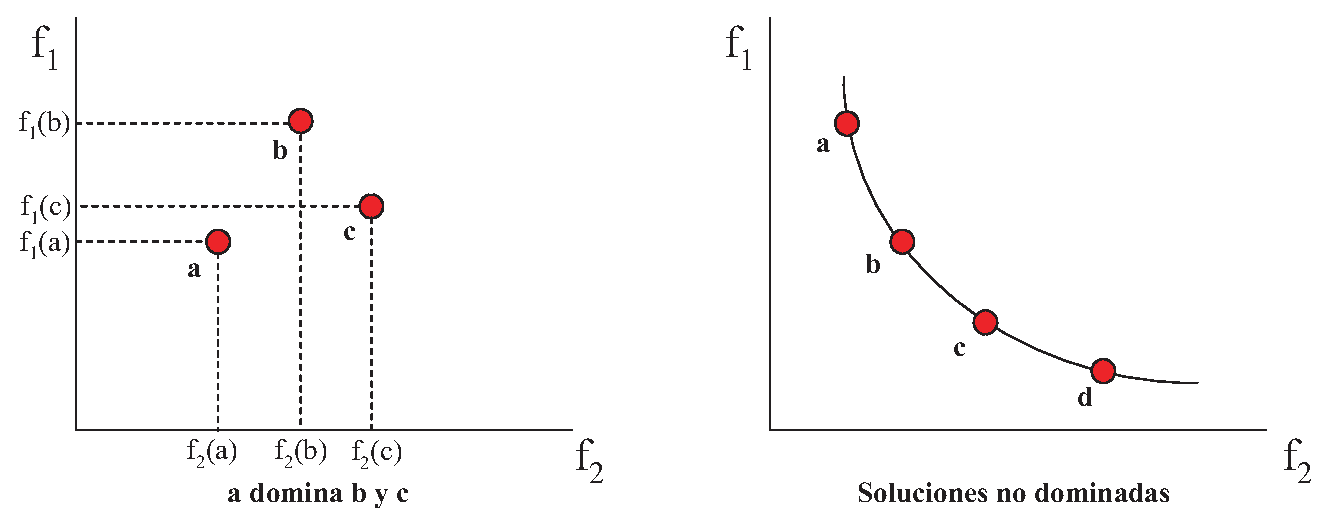
\epsfig{file=./img/metaheuristics/dominancia, width=14cm}
	\caption{Pareto dominance example.} \label{fig:decisions_objective_space}
\end{figure} 
The precedent definition applies for global Pareto optimality however, also local Pareto optimality may be defined. A decision vector $x^{*} \in S$ is locally Pareto optimal if there exists a neighborhood $N(x^{*})$ of $x^{*}$ such that $x^{*}$ is Pareto optimal in $N(x^{*}) \cap S$. The objective vector $f(x^{*})$ is locally Pareto optimal if the corresponding point $x^{*}$ is locally Pareto optimal.
 
The concept of dominance is related to Pareto optimality. In \ref{fun:mop}, an objective vector $z^{1}$ is said to \textit{dominate} another vector $z^{2}$ if $z_{i}^{1} \leq z_{i}^{2} $ for all $i= 1,...,k$, and the inequality is strict for least on index $i$.Furthermore, an objective vector $z^{1}$ is \textit{non-dominated} if there does not exist another objective vector $z^{2}$ such $z^{2}$  dominates $z^{1}$, therefore, Pareto optimal points are non-dominate points. Figure \ref{fig:dominance} shows the concepts of dominance and non-dominance.
\begin{figure}[H] %t
	\centering 
	\includegraphics[width=0.80\textwidth]{figures/metaheuristics/my-dominance.png}
	%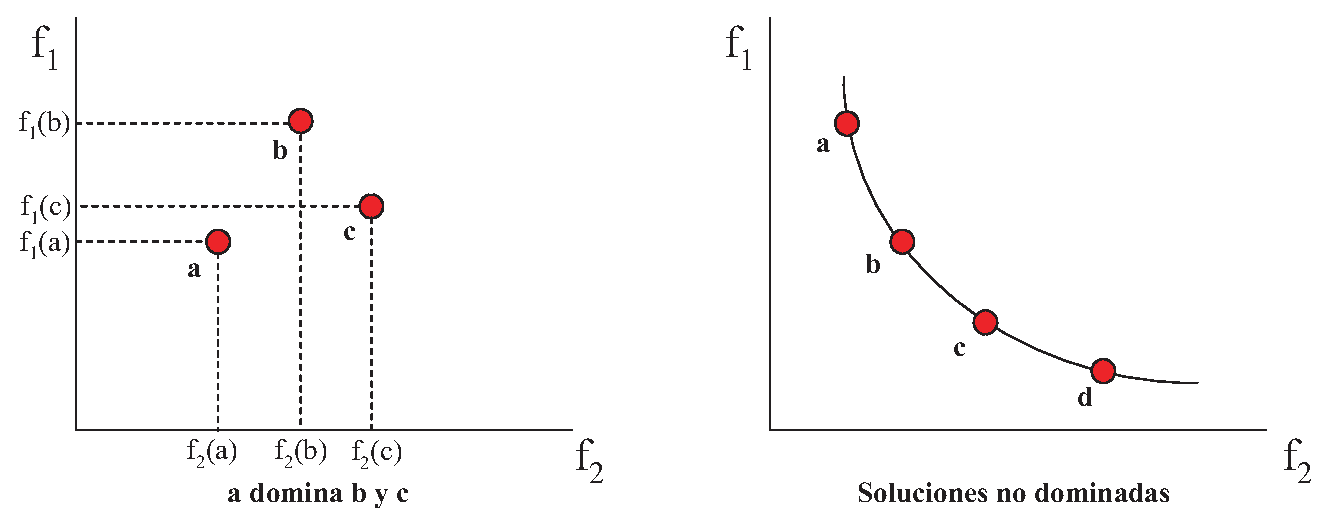
\epsfig{file=./img/metaheuristics/dominancia, width=14cm}
	\caption{Pareto dominance example.} \label{fig:dominance}
\end{figure} 

The limits of objective function values in the Pareto optimal front (called Pareto front) are defined by \textit{ideal} and \textit{nadir} objective vectors. An ideal objective vector $z^{*} \in \mathbb{R}^{k}$ gives lower bounds for the objective functions, and it is obtained by minimizing each objective function individually subject to the constraints. A vector strictly better than $z^{*}$ can be called a\textit{utopian objective vector} $z^{**}$ therefore thus, we set $z_{i}^{**} = z_{i}^{*}- \epsilon$ for $i = 1,...,k$, where $\epsilon$ is a small positive integer. Finally, a \textit{nadir objective vector} $z^{nad}$ is the upper bounds of objective function values in the Pareto optimal set, it is not easy to calculate; consequently, these values are usually only approximated for instance, by using pay-off tables \cite{deb2010nadir,miettinen1999nonlinear}. Examples of ideal, utopian and nadir objective vectors are shown in Figure \ref{fig:ideal_nadir}. Since there exist many Pareto optimal solutions, a decision maker is needed for choosing one solution among them. A decision maker (DM) is a person who is an expert in the domain of the multi-objective optimization problem and can express her/his preference information to choose the most preferred solution.
A very popular type of preference articulation in multi-objective methods is based on \textit{reference points} \cite{branke2008multiobjective,kaisa2016}, which represent the region of interest in the form of desirable objective function values. A reference point is regarded as an intuitive way to express preferences. However, such methods are regarded as ad hoc methods, i.e., methods where the DM cannot be replaced by a value function~\cite{miettinen1999nonlinear,Stewart2005}. 

\begin{figure}[H] %t
	\centering 
\includegraphics[width=0.80\textwidth]{figures/multiobjective/vector_ideal_nadir.png}
	%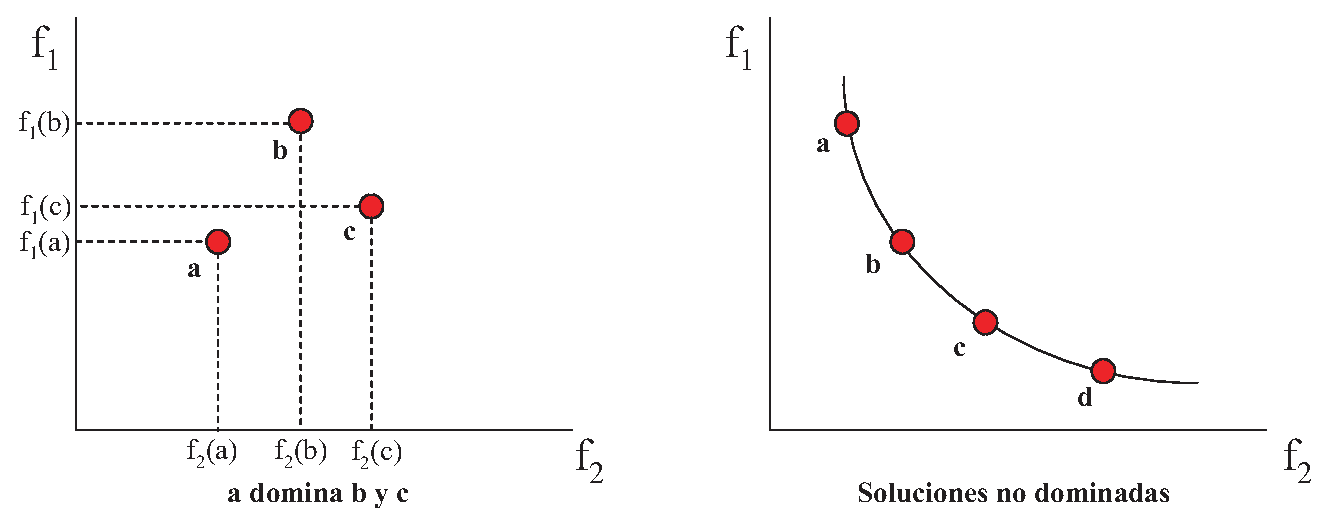
\epsfig{file=./img/metaheuristics/dominancia, width=14cm}
	\caption{Ideal, utopian and nadir objective vectors} \label{fig:ideal_nadir}
\end{figure} 

\section{Classification of multi-objective methods}
The techniques used to solve MOPs are not usually restricted to finding a single solution, but a set of compromise solutions between the multiple conflicting objectives, since there is usually no solution that simultaneously optimizes all objectives. Two stages can therefore be distinguished when addressing this type of problem: on the one hand, the optimization of several objective functions involved and, on the other hand, the decision-making process on which compromise solution is most appropriate \cite{coello07evolutionary}. Multi-objective optimization methods can be classified according to the role of the decision maker in the solution process.  \cite{cohon75review}:

\begin{itemize}
	\item \emph{No-preference methods}: This methods are usually used when there is no DM available or when no preference information from the DM us available consequently, the opinions of the DM are not taken into consideration.
	\item \emph{A posteriori methods}: In this methods the exploration is made as wide as possible to generate as many compromise solutions as possible. It is, then, when the decision-making process by the expert takes place. Precisely, because of this approach, these \emph{a posteriori} techniques are being used in the field of metaheuristics and, particularly, in the field of evolutionary computing \cite{coello07evolutionary, deb01multiobjective}. More specifically, the most advanced algorithms apply \emph{a posteriori} techniques based on the concept of \emph{Pareto Optimality} \cite{pareto96cours}.
	\item \emph{A priori methods}: In this methods, the DM specifies his/her preferences before the solution process. The main withdraw of this method is that DM does not necessarily know beforehand whether the solutions will be realistic. Lexicographic ordering \cite{fishburn1974exceptional} and goal programming \cite{charnes1977goal,charnes1955optimal} are examples of a priori methods.
    \item \emph{Interactive methods}: In interactive methods, the DM articulates preference information iteratively and thus directs the solution process progressively.Only part of the Pareto optimal set has to be generated and evaluated, and based on this data the DM can further adjust his/her preferences as the solution process continues. The procedure is iterated until the DM is satisfied with the Pareto optimal solution. The advantage of using interactive methods is that the DM can guide the solution process and simultaneously learn about the different trade-offs between different solutions. In the last decades, many interactive methods have been proposed such as, Step method \cite{benayoun1971linear}, reference point method \cite{wierzbicki1980use}, satisficing trade-off method \cite{nakayama1984satisficing}, NIMBUS method \cite{miettinen1995interactive}, etc. Recently, several evolutionary algorithm based interactive methods have also proposed, such as progressively interactive evolutionary multi-objective algorithm \cite{deb2010interactive,nebro2018indm2,fowler2010interactive,phelps2003interactive} or interactive territory defining evolutionary algorithm \cite{koksalan2010interactive}.
\end{itemize}

There exists other ways for classifying the multi-objective methods, such as 


-algoritmos dinamicos vs algoritmos estaticos
-hablar de metaheuristics


   


\chapter{jMetalSP} % Main chapter title

\label{chaper:jmetalsp} % Change X to a consecutive number; for referencing this chapter elsewhere, use \ref{ChapterX}

%----------------------------------------------------------------------------------------
%	SECTION 1
%----------------------------------------------------------------------------------------

\section{Introduction}
Currently, the growing interest in Big Data applications~\cite{BD-challenges-2014}, where many of them require to process large amounts of data coming at great speed from streaming data sources, brings new opportunities to apply dynamic multi-objective optimization. The rationale is that both, Big Data and multi-objective optimization are found in many disciplines, such as: transportation, economics,
mobility, and medicine; so it is foreseeable that they converge in a near future leading to multi-objective Big Data optimization problems. 


% Descripción de la metodología seguida
%\chapter{Methodology}
\label{chapter:methodology}
\index{Methodology}

In this chapter, we present the tools we have used for our study. First, we discuss a little the concepts about AutoDock, the software used to solve the molecular docking problem. Then, we present the jMetal framework, used to include new different metaheuristic techniques into the AutoDock software. Finally, we explain how the integration between the two software tools was done.

\section{AutoDock}
\index{AutoDock}

%TODO: Incluir mucha más información sobre AutoDock

AutoDock is a suite of automated docking tools. This software has been designed to predict how small molecules, such as substrates or drug candidates, bind to a receptor of known 3D structure. AutoDock actually consists of two main programs: {\it autodock} which performs the docking of the ligand-protein and {\it autogrid} which pre-calculates the grids of interaction of ligand-protein complex.

The last version of AutoDock used in this study is the version 4.2. Since this version, AutoDock allows sidechains in the macromolecule to be flexible. It also included a free-energy scoring function (which has been used by the metaheuristics of this study) that is based on a linear regression analysis, the AMBER force field, and an even larger set of diverse protein-ligand complexes with known inhibition constants.

In addition to using them for docking, the atomic affinity grids can be visualized. This can help, for example, to guide organic synthetic chemists design better binders. AutoDock has applications in X-ray crystallography, structure-based drug design, lead optimization, virtual screening (HTS), combinatorial library design, protein-protein docking and chemical mechanism studies.

AutoDock 4 is a free software and is available under the GNU General Public License.

\section{The jMetal framework}

jMetal was designed following an object-oriented architecture which facilitates the inclusion of new components and the reuse of existing ones. It provides the user with a set of base classes which can be used to design new algorithms, and to implement problems or complex operators, etc. This section is aimed at describing the classes composing the core of jMetal. %When applicable, we will establish an analogy between the class and the corresponding concept in the field of evolutionary algorithms. 

Figure~\ref{fig:architecture} depicts an UML diagram including the base classes within jMetal.
The working principle of jMetal is based in relies in that an {\it Algorithm} solves a {\it Problem} using one (and possibly more) {\it SolutionSet} and a set of {\it Operator} objects. As we can see in the figure, the tool contains classes for representing those and some other elements.

\begin{figure*}[!h]%figure_architecture
	\centerline{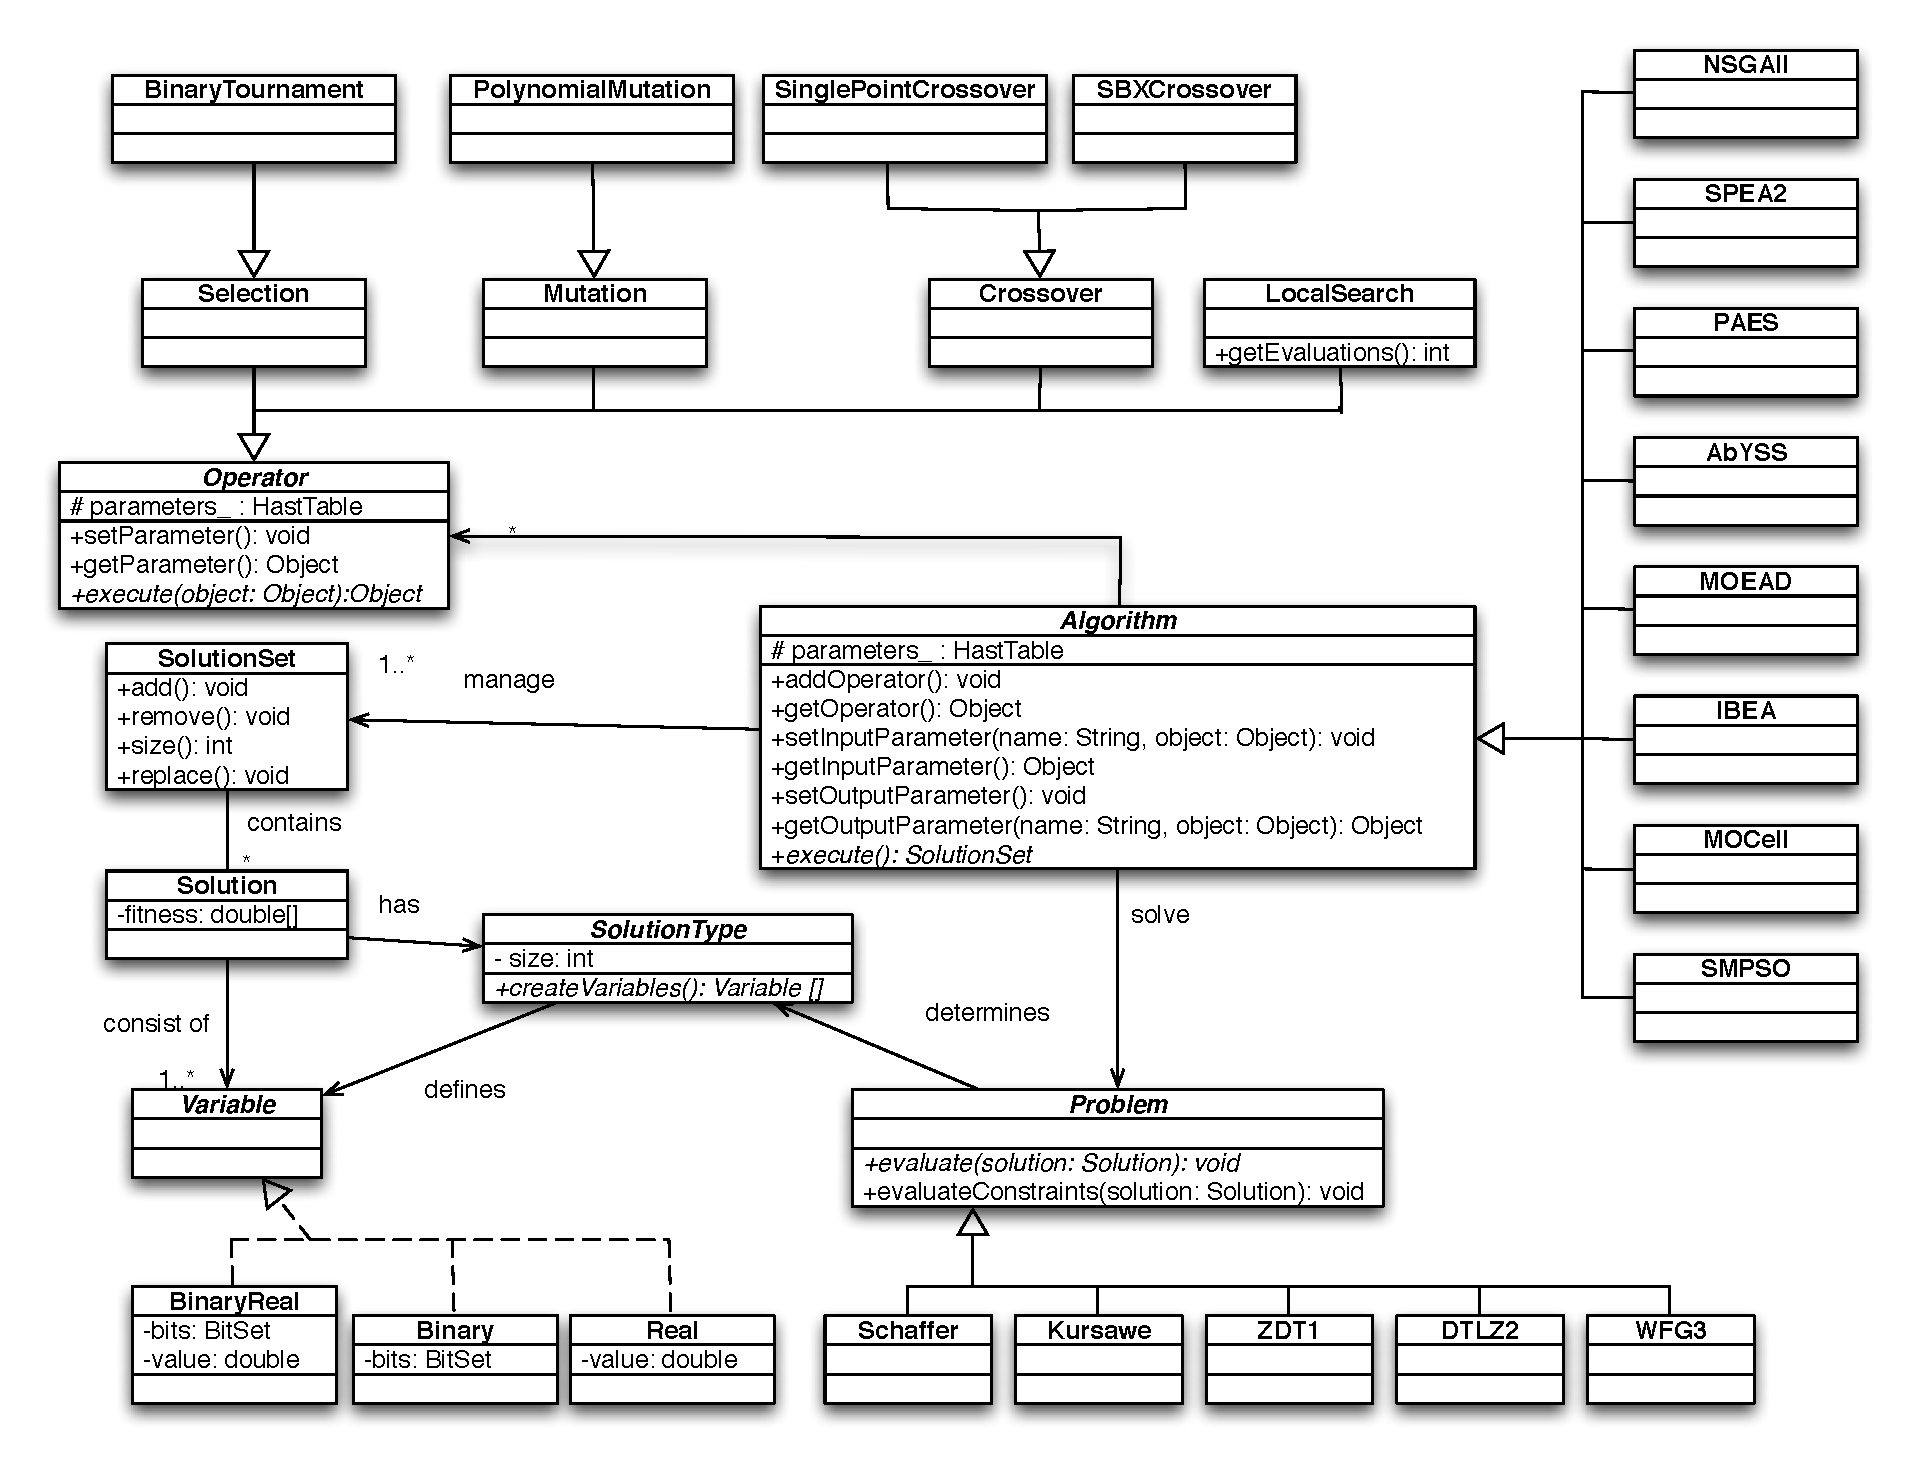
\includegraphics[width=135mm]{img/methodology/jMetalUML.eps}}
	\caption{General architecture of jMetal.}
	\label{fig:architecture} 
\end{figure*}

A generic terminology to name the classes within jMetal was employed in order to make them general enough to be used in any metaheuristic. This way, in the context of evolutionary algorithms, populations and individuals correspond to {\it SolutionSet} and {\it Solution} jMetal classes, respectively; the same can be applied to PSO algorithms concerning the concepts of swarm and particles.

Class {\it Algorithm} represents the superclass for all the optimizers: whatever metaheuristic included in jMetal has to inherit from it. An instance object of {\it Algorithm} may require some application-specific parameters, that can be added and accessed by using the methods {\it addParameter()} and {\it getParameter()}, respectively. Similarly, an algorithm may also make use of some operators. For example, genetics algorithms typically use operators for recombination and selection of individuals. There are also methods for incorporating operators ({\it addOperator()}) and to get them ({\it getOperator()}). The main method in {\it Algorithm} is {\it execute()}, which starts the execution of the algorithm. 

As its name suggests, class {\it SolutionSet} represents a set of {\it Solution} objects. Each {\it Solution} object has associated a type ({\it SolutionType}) and it is composed of an array of {\it Variable} objects. This last is a superclass aimed at describing different kinds of representations for solutions. The proposed scheme by jMetal is very flexible because a {\it Solution} object is not restricted to contain variables of the same representation; instead, it can be composed of an array of mixed variable types. Furthermore, it is also extensible, because new representations can be easily incorporated into the framework, just by inheriting from {\it Variable}.

In jMetal, all the problems have to inherit from class {\it Problem}. This class contains two basic methods: {\it evaluate()} and {\it evaluateConstraints()}. Both methods receive a {\it Solution} representing a candidate solution to the problem; the first one evaluates it, and the second one determines the overall constraint violation of that solution. All the problems have to define the {\it evaluate()} method, while only problems having side constraints need to define {\it evaluateConstraints()}. The constraint handling mechanism implemented by default is the one proposed in~\cite{deb02fast}.

{\it Operator} is a superclass aimed at representing generic operators to be used by the different algorithms (e.g., crossover, mutation, or selection are typical operators in the field of evolutionary algorithms). As {\it Algorithm}, it contains the {\it getParameter()} and {\it setParameter()} methods, which are used for adding and accessing to operator specific parameters. For example, the simulated binary (SBX) crossover~\cite{deb01multiobjective}, employed by many evolutionary algorithms, requires two parameters: a crossover probability (as most crossover operators) plus a value for the distribution index (specific of the parameter). This operator receives as a parameter two parent individuals and, as a result, it returns the offspring resulting of recombining both parents. The use of the generic Java class {\tt Object} allows a high degree of flexibility. Thus, a {\it BinaryTournament} operator, which is a selection operator employed by many genetic algorithms, will receive as a parameter a {\it SolutionSet} object and it will return a {\it Solution} object, while a {\it PolynomialMutation} operator, also a mutation operator typically used in evolutionary algorithms, will receive a {\it Solution} object, will modify this object, and it will return a null value.

A more detailed description of the jMetal architecture can be found in~\cite{DN10jmetal} and in the jMetal user manual~\cite{ND10}.

\section{Integrating jMetal and AutoDock 4.2}
\label{sec:jMetal_Autodock}

jMetal is an open-source framework aimed at multi-objective optimization with metaheuristics, but it also incorporates many algorithms for single-objective optimization. Our idea is to develop a clean integration between jMetal and AutoDock 4.2 in such a way that the algorithms available in jMetal can be used to solve docking problems by using the fitness function provided by AutoDock 4.2 (in the case of mono-objective metaheuristics). This implies that the metaheuristics run in jMetal and, whenever a new solution has to be evaluated, the solution has to be sent to AutoDock, which returns the corresponding binding energy. Once AutoDock has been properly configured, it enters a loop and waits for jMetal evaluation requests; when the algorithm in jMetal finishes, the best solution is sent to AutoDock, which continues its execution as if the incorporated GA or LGA had finished (see Figure~\ref{Fig:integration}). Thus, the final results have the same format and they are familiar to AutoDock users.

\begin{figure*}[!h]%figure_integration
	\centerline{\includegraphics[width=0.70\textwidth]{img/methodology/integration.png}}
	\caption{Sequence diagram which represents the communication between AutoDock and jMetal during a mono-objective algorithm execution. The two threads communicate with each other a number of times, equal to the number of evaluations. Finally, the jMetal thread returns the best solution to the main AutoDock thread.}
	\label{Fig:integration} 
\end{figure*}

In the case of the multi-objective metaheuristics, the integration process is nearly identical but differs in some small details. Instead of getting the binding energy value (fitness) after sending a solution to AutoDock to be evaluated, the code was modified to receive to independents components of that binding energy value: the intermolecular energy and the intramolecular energy. These two values will be treated as two different objectives to be minimized. After finishing all the algorithm iterations, instead of getting one best solution, a front containing a set of non-dominated solutions is obtained. However, one of the solutions contained in the front has to be returned to the AutoDock thread, so the main thread is able to finish as expected (see Figure~\ref{Fig:integration-multi}).

\begin{figure*}[!h]%figure_integration_multi
	\centerline{\includegraphics[width=0.70\textwidth]{img/methodology/integration-multi.png}}
	\caption{Sequence diagram which represents the communication between AutoDock and jMetal during a multi-objective algorithm execution. The two threads communicate with each other a number of times, equal to the number of evaluations. Finally, the jMetal thread returns a non-dominated solution to the main AutoDock thread. The entire approximated front is returned by the jMetalCpp thread in an output file.}
	\label{Fig:integration-multi} 
\end{figure*}

In our first attempt, we considered using the JNI framework to directly invoke the AutoDock energy function from jMetal, but AutoDock 4.2 is a rather complex software package, which requires the parameter settings of an experiment to be indicated in a configuration file, and a pre-processing of them is required in order to start running a solver. We therefore decided that a more promising approach was to first configure both packages and then run them in parallel.

As jMetal and AutoDock are coded in different languages, the first integration was done by using sockets for the communication between them; JSON was used as data interchange format. This solution worked, but it was very inefficient, so we took the decision to write a port of a significant subset of jMetal to C++ from scratch. The adopted solution consists of running AutoDock and jMetal in two different threads inside the same process, so they communicate by sharing memory and synchronize with mutexes (see Figure~\ref{Fig:integration} and Figure~\ref{Fig:integration-multi}). This approach is efficient and flexible, allowing any of the algorithms included in jMetal to be easily used for solving docking problems.
% Capítulo sobre Web Semántica
\chapter{Web Semantic} % Main chapter title

\label{ChapterWebSemantic} % Change X to a consecutive number; for referencing this chapter elsewhere, use \ref{ChapterX}

%----------------------------------------------------------------------------------------
%	SECTION 1
%----------------------------------------------------------------------------------------

\section{Introduction}
% Papers del compendio
\chapter{Published Work}
\label{chapter:publishedWorks}
\index{Published work}

We have published several research studies based on the application to multi-objective metaheuristics to solve the molecular docking problem. Specifically, four articles have been published in journals indexed in the Journal of Citation Report (JCR) from the Institute of Scientific Information. In addition to this, four articles have been published in congresses. Two of them have been published in international congresses and the rest in national congresses.

\section{List with Research Contributions}

These four JCR articles apply metaheuristics to solve the molecular docking problem. These contributions can be organized as follows:\\

\noindent \textbf{Articles published in journal indexed in JCR:}

\begin{itemize}[leftmargin=5.5mm]
	
	\item \fullcite{lopez14jmetalcpp}\\Impact Factor: 4,981. Q1 (3/57)  in the category of mathematical and computational biology.
	
	\item \fullcite{lopez2015asoc}\\Impact Factor: 2,857. Q1 (21/130) in the category of Computer Science and Artificial Intelligence.
	
	\item \fullcite{Molecules2015}\\Impact Factor: 2,465. Q2 (25/59) in the category of Chemistry, Organic.
	
	\item \fullcite{Molecules2016}\\Impact Factor: 2,465. Q2 (25/59) in the category of Chemistry, Organic.
	
\end{itemize}

\noindent \textbf{Articles published in international congresses:}

\begin{itemize}[leftmargin=5.5mm]
	
	\item \fullcite{LopezCamacho2016AlCoB}
	
	\item \fullcite{GarciaNieto2016ANTS}

\end{itemize}

\noindent \textbf{Articles published in national congresses:}

\begin{itemize}[leftmargin=5.5mm]
	
	\item \fullcite{lopez2015maeb}
	
	\item \fullcite{lopez2016maeb}  

\end{itemize}

\section{Summary of the articles that support the thesis}
\label{sec:Summary_articles_support}

This section summarizes the articles that support this thesis. All these papers are related to the application of the single-objective and multi-objective optimizations to solve the problem of the molecular docking. In the first article, we have described the integration of AutoDock and jMetal and its application in the domain of molecular docking. In the second published article, we have performed a study comparing the mono-objective techniques using a set of flexible instances. In a third and fourth study, we have applied a set of multi-objective metaheuristics that optimize two objectives, guiding the algorithm to search the best molecular docking solutions.

\subsection{jMetalCpp: optimizing molecular docking problems with a C++ metaheuristic framework}

\textbf{Reference:}~\cite{lopez14jmetalcpp} \fullcite{lopez14jmetalcpp}\\
Pages in this thesis: \pageref{start-pdf/bioinformatics.pdf}-\pageref{stop-pdf/bioinformatics.pdf}

In~\cite{lopez14jmetalcpp} we introduced jMetalCpp, the C++ version of the metaheuristic framework jMetal (originally written in Java). We also presented the combination of this software with the widely used AutoDock, which is the most used tool to solve molecular docking problems. The inclusion of jMetalCpp inside the AutoDock provided the latter several additional metaheuristic techniques to solve molecular docking problems. Both new softwares (the standalone jMetalCpp and the ``fusion'' of jMetalCpp with AutoDock) were published online\footnote{http://jmetalcpp.sourceforge.net/}$^{,}$\footnote{http://khaos.uma.es/autodockjmetal/} to be freely used by the scientific community.

\subsection{Solving molecular flexible docking problems with metaheuristics: a comparative study}

\textbf{Reference:}~\cite{lopez2015asoc} \fullcite{lopez2015asoc}\\
Pages in this thesis: \pageref{start-pdf/asoc.pdf} -- \pageref{stop-pdf/asoc.pdf}

In our first single-objective study~\cite{lopez2015asoc}, we tested the performance of new metaheuristic techniques apart from those included in the AutoDock Tools for solving molecular docking problems. This study approached the problem as a single-objective optimization problem, as AutoDock does. AutoDock provides two different techniques to solve the problem: a Lamarckian Genetic Algorithm (LGA), which includes local search, and a common Genetic Algorithm (GA). We added four single-objective metaheuristic: generational Genetic Algorithm (gGA), steady-state Genetic Algorithm (ssGA), Differential Evolution (DE) and Particle Swarm Optimization (PSO). A study with 75 protein-ligan complexes taken from PDB was carried on using the same fitness function and configuration parameters than AutoDock to have a comparison as fair as possible. The objective was the binding energies in kcal/mol associated with the receptor-ligand complex, as explained in Section~\ref{subsection:mono_solution}. Therefore, the lower the binding energy the better the result.

This study had two different steps. In the first one, we tuned the parameter configuration of the four single-objective metaheuristic techniques. In order to do so, we selected 11 protein-ligand complexes taken from the PDB database. After we obtained a set of configuration parameters for the 4 single-objective metaheuristics, a thorough comparison was made between these four and the algorithms provided by AutoDock. This time, a set of 75 instances also from PDB were used.

It was demonstrated that DE (jMetal) obtained the best results in 67 of the 75 instances, followed by LGA (AutoDock) that achieved the best results in the remaining eight instances (1B6L, 1BDL, 1HEF, 1HIV, 1HPO, 1K6C, 1Z1H and 1ZIR). These results were provided with statistical confidence ($\alpha = 0.05$) as a series of non-parametric statistical tests were applied. In particular, Friedman's ranking and Holm's post-hoc multicompare tests were calculated and showed that DE achieved a statistically better performance than the rest of the other analyzed algorithms. This fact is remarkable as the AutoDock algorithms are specifically designed to solve molecular docking problems.
It was also noted that DE showed a slower convergence behavior, though with more successful solutions than its competitors. However, gGA demonstrated a fast convergence, and also achieved high-quality solutions, so this algorithm could be a good choice when looking for fast, but good enough solutions.

\subsection{A new multi-objective approach for molecular docking based on RMSD and binding energy}

\textbf{Reference:}~\cite{LopezCamacho2016AlCoB} \fullcite{LopezCamacho2016AlCoB}\\
Pages in this thesis: \pageref{start-pdf/alcob.pdf} -- \pageref{stop-pdf/alcob.pdf}

This work was presented in the 3rd International Conference on Algorithms for Computational Biology (AlCoB 2016), celebrated in Trujillo, Spain in June of 2016. It was derived from the idea of taking a multi-objective optimization approach to solve molecular docking problems. In the beginning, the strategy we had followed was to decompose the final binding energy (the minimization objective of the previous work) into several components, particularly the intra- and inter-molecular energy~\cite{Molecules2015}. After that, it was decided to use as objectives the same energy taken in the single-objective study and the RMSD. These concepts were explained in more detail in Section~\ref{subsection:multi_solution}.

However, in this paper~\cite{LopezCamacho2016AlCoB}, we selected four representative multi-objective optimization algorithms such as NSGA-II, GDE3, SMPSO and MOEA/D. A benchmark composed of 11 complexes having receptor and ligand flexibility was selected. The selection of these complexes was motivated as they are docking problems containing a wide range of ligand sizes (from small to large inhibitors). Two quality indicators were calculated to measure the performance of each algorithm: Hypervolume (I$_{HV}$) and Unary Additive Epsilon Indicator ($I_{\epsilon+}$). The first indicator takes into account both convergence and diversity, whereas the second one ($I_{\epsilon+}$) gives a measure of the convergence degree of the obtained Pareto front approximations. It is worth noting that, as we are dealing with real-world optimization problems, the true Pareto fronts needed to calculate these metrics are not known, so they had to be obtained using all the approximated fronts from all the executions of all the multi-objective algorithms for each problem.

The $I_{HV}$ is the sum of the contributed volume of each point of a front in respect to a reference point, so the higher the convergence and diversity degrees of a front, the higher its $I_{HV}$ value. According to these results, SMPSO achieved the best $I_{HV}$ values in all the eleven problems, being MOEA/D the second best performing technique. It is important to note that many algorithms had a $I_{HV}$ value equal to zero, this happens when all the points of the produced fronts are beyond the limits of the reference point. This happened in most of the problems in all the algorithms excepting SMPSO, what leaded us to think that we are facing a hard optimization problem.
Also, SMPSO achieved the best performance results according the $I_{\epsilon+}$ indicator (in this case, the lower the value, the better). SMPSO achieved the best values for all 11 instances except for 1HTF, in which it got the second best value. MOEA/D, which was the algorithm that got the best value for 1HTF, achieved the second best values for 9 instances. GDE3 got the second best value in one instance (1HPX) while NSGA-II got the worst results for all the instances.

After this work was presented, it was invited to be substantially extended and be submitted to a special issue of the journal IEEE/ACM Transactions on Computational Biology and Bioinformatics (TCBB, 2014 JCR impact factor: 1.438, quartile Q1). To this day, it is still under-review.

\subsection{A study of archiving strategies in multi-objective PSO for molecular docking}

\textbf{Reference:}~\cite{GarciaNieto2016ANTS} \fullcite{GarciaNieto2016ANTS}\\
Pages in this thesis: \pageref{start-pdf/ants.pdf} -- \pageref{stop-pdf/ants.pdf}

This work~\cite{GarciaNieto2016ANTS} was presented in the 10th International Conference on Swarm Intelligence (ANTS 2016), celebrated in Brussels, Belgium in September of 2016. It is the natural continuation from the previous one, where we obtained that SMPSO obtained best overall results when applying a multi-objective approach to solve molecular docking problems. The previous experiment was replicated using several SMPSO variants based on different archiving strategies. The selected variants are: SMPSO$_{hv}$, SMPSOD and SMPSOC. The original SMPSO and OMOPSO (the algorithm which SMPSO was inspired from) were also included in the comparison.

This paper introduced the variant named SMPSOC. It is characterized by the use of a cosine similarity when calculating the density value of each point in the solution front. The variant SMPSOD was also presented in this paper for the first time. It is an archive-less approach, implemented as an aggregative version of SMPSO inspired by MOEA/D.

According to the $I_{HV}$ indicator, SMPSO$_{hv}$ obtained the best results for all the 11 instances, whereas SMPSOD got the second best value in 6 instances, SMPSOC in three and the original SMPSO in two, respectively. In the same manner, SMPSO$_{hv}$ obtained again the best values for the 11 instances according to the $I_{\epsilon+}$ indicator. The second best values were achieved by SMPSOD in 7 instances, the original SMPSO in three and SMPSOC in one instance, respectively.

\section{Summary of other publications related to this thesis}

This section briefly comments the other four articles that do not support this thesis but are related to its topic. Two of them were published in the Molecules journal and the other two were published in national congresses.

In \cite{Molecules2015}, we presented our first multi-objective approach. The final binding energy (the minimization objective of the mono-objective study) was decomposed into the intra- and inter-molecular energy. These two components were used as two contrary objectives. We selected six multi-objective optimization algorithms such as NSGA-II, ssNSGA-II, GDE3, SMPSO, MOEA/D and SMS-EMOA. A heterogeneous set of 11 protein-ligand complexes with flexible ligands and receptors was selected in order to carry out the experiments. A use case of drug discovery that involves the aeroplysinin-1 compound and the human Epidermal Growth Factor (EGFR) was also provided. The results demonstrated that according to the use casses presented, it can be more interesting to select a specific docking solution with a balanced tradeoff between the E$_{inter}$ and E$_{intra}$ values.

In \cite{Molecules2016}, we presented our latest multiobjective approach. This time, we selected the final binding energy and the RMSD as optimization objectives and NSGA-II, GDE3, SMPSO and MOEA/D as multi-objective optimization algorithms. In this study, we performed an analysis on binding sites in the EGFR kinase domain and molecular interactions. The use cases were based on instances with wild-type EGFR, EGFR with mutations L858R and G719S and EGFR double mutants (T790M/L858R and T790M/G719S). This proposed approach can be used for in silico studies to test other analog kinase inhibitors or similar compounds for drug discovery in those cancers in which therapeutic targets are changed by somatic mutations.

The two latter articles where published in the X and XI `Congreso Español de Metaheurísticas, Algoritmos Evolutivos y Bioinspirados (MAEB)' in 2015 and 2016. The first article \cite{lopez2015maeb} presented our first multi-objective approach (using the intra- and inter-molecular energy as contrary objectives). The following year, we presented our multi-objective PSO study in this same congress \cite{lopez2016maeb}.

\section{Copies of the articles that support the thesis}

This section includes copies of the four articles summarized in Section \ref{sec:Summary_articles_support}

\includepdf[pages=-,scale=0.83,pagecommand={\pagestyle{fancy}}]{pdf/bioinformatics.pdf}

\includepdf[pages=-,scale=0.83,pagecommand={\pagestyle{fancy}}]{pdf/asoc.pdf}

\includepdf[pages=-,scale=0.80,pagecommand={\pagestyle{fancy}}]{pdf/alcob.pdf}

\includepdf[pages=-,scale=0.80,pagecommand={\pagestyle{fancy}}]{pdf/ants.pdf}


%Resumen global de los resultados
%\chapter{Results}
\label{chapter:results}
\index{Results}

In this chapter, we show a global summary of all the results obtained in the published works that sustain this dissertation. First, in Section~\ref{sec:SingleObjectiveStudy} we will summarize the results obtained in our single-objective study. Then, in Section~\ref{sec:MultiObjectiveStudy}, the results obtained in the multi-objective works will be shown and discussed briefly.

\section{Single-objective study}
\label{sec:SingleObjectiveStudy}

In our first single-objective study~\cite{lopez2015asoc}, we tested the performance new metaheuristic techniques apart from those included in the AutoDock Tools for solving molecular docking problems. This study approached the problem as a single-objective optimization problem, as AutoDock does. AutoDock provides two different techniques to solve the problem a Lamarckian Genetic Algorithm (LGA), which includes local search, and a common Genetic Algorithm (GA). We added four single-objective metaheuristic: generational Genetic Algorithm (gGA), steady-state Genetic Algorithm (ssGA), Differential Evolution (DE) and Particle Swarm Optimization (PSO). A study with 75 protein-ligan complexes taken from PDB was carried on using the same fitness function and configuration parameters than AutoDock to have a comparison as fair as possible.

In Table~\ref{tab:asoc-medians-75}, the median binding energy (the fitness function used in this study) of the six compared algorithms (four from jMetal and two from AutoDock) from 30 independent runs for each one of the 75 analyzed molecules. These binding energies in kcal/ml associated with the receptor-ligand complex, as explained in Section~\ref{subsection:mono_solution}. Therefor, the lower the binding energy the better the result.

In Table~\ref{tab:asoc-medians-75}, the best result for each instance is marked with a gray background. With a first observation, it is noticeable that DE (jMetal) obtained the best results in 67 of the 75 instances, followed by LGA (AutoDock) that achieved the best results in the remaining eight instances (1B6L, 1BDL, 1HEF, 1HIV, 1HPO, 1K6C, 1Z1H and 1ZIR). These results were provided with statistical confidence ($\alpha = 0.05$) as a series of non-parametric statistical tests were applied. In particular, Friedman's ranking and Holm's post-hoc multicompare tests were calculated and showed that DE achieved a statistically better performance than the rest of the other analyzed algorithms. This fact is remarkable as the AutoDock algorithms are specifically designed to solve molecular docking problems.
It was also noted that DE showed a slower convergence behavior, though with more successful solutions than its competitors. However, gGA demonstrated a fast convergence, and also achieved high-quality solutions, so this algorithm could be a good choice when looking for fast, but good enough solutions. More details about this study are presented in section~\ref{sec:publications-asoc} and its correspondent publication.

\begin{table}
	\caption{\label{tab:asoc-medians-75}Performance results of compared algorithms (gGA, ssGA, DE, and PSO from jMetal; GA and LGA from AutoDock) for the test set of 75 docking instances. Each cell contains the median binding energy values (kcal/mol) from 30 independent runs for each molecule (with PDB accession code) and algorithm}
	\scriptsize
	\centering
	\begin{tabular}{ll|rrrrrrrrrrrrrrrrrrrr}
		\hline			
		Algs./ & PDB	 & 1A94 & 	1A9M	 & 1AAQ	 & 1B6J & 	1B6K & 	1B6L & 	1B6P & 	1B6M & 	1BDL & 	1BDQ\\
		\hline
		\multirow{4}{*}{jMetal} &   gGA	 & 2.72	 & 0.075 & 	-0.83 & -2.23 & -2.49 & -3.915 & 	-3.365 & 	-3.61 & 	-0.965 & 	-1.145 \\
		\multirow{4}{*}{} &        ssGA & 	4.1 & 	0.755 & 	0.13 & 	-0.685 & -2.285 & -2.89 & -2.28 & 	-2.435 & 	-0.4 & 	0.375\\
		\multirow{4}{*}{} &          DE	 &\cellcolor{gray25} 0.7 &\cellcolor{gray25} 	-3.18 &\cellcolor{gray25} 	-1.865 & \cellcolor{gray25}	-3.885 &\cellcolor{gray25} 	-5.26 & 	-6.04 &\cellcolor{gray25} 	-6.985	 &\cellcolor{gray25} -5.865 & 	-2.275 &\cellcolor{gray25} 	-3.09\\
		\multirow{4}{*}{} &          PSO	 & 5.545	 & 1.785	 & 1.025 & 	-0.43	 & -0.965 & 	-2.83	 & -1.6	 & -1.08	 & 0.755	 & 0.975\\
		\hline
		\multirow{2}{*}{ADock} &          GA	 & 4.35	 & 1.56 & 	0.785	 & -0.575	 & -1.33 & 	-3.505 & 	-2.445 & 	-2.49 & 	0.415 & 	0.27\\
		\multirow{2}{*}{} &         LGA & 	1.41	 & -1.695	 & -1.8	 & -3.45 & 	-4.83 & \cellcolor{gray25}	-6.27 & 	-5.285 & 	-5.155 & \cellcolor{gray25}	-2.36 & 	-2.64\\
		
		\hline
		\hline			
		Algs./ & PDB & 1BDR &	1BV7 &	1BV9 &	1BWA &	1BWB &	1D4K &	1D4L &	1DMP &	1G35 &	1GNM\\
		\hline
		\multirow{4}{*}{jMetal} &  gGA	 & -1.895&-3.345&-4.105&-2.14&-2.96&-6.33&-6.805&-2.99&-3.21&-3.145\\
		\multirow{4}{*}{} &           ssGA & 	-0.27&-2.18&-2.19&-2.715&-1.955&-4.235&-4.95&-1.885&-2.065&0.85\\
		\multirow{4}{*}{} &           DE	 &\cellcolor{gray25} -2.83&\cellcolor{gray25}-6.13&\cellcolor{gray25}-5.8&\cellcolor{gray25}-5.47&\cellcolor{gray25}-5.345&\cellcolor{gray25}-8.135&\cellcolor{gray25}-9.45&\cellcolor{gray25}-5.605&\cellcolor{gray25}-5.43&\cellcolor{gray25}-4.4\\
		\multirow{4}{*}{} &            PSO	 & 0.315&-1.14&-0.81&-0.7&-0.46&-2.21&-2.52&-1.06&-0.965&2.165\\
		\hline
		\multirow{2}{*}{ADock} &            GA	 & 0.18&-1.715&-2.09&-1.725&-1.69&-4.09&-4.25&-1.725&-1.55&0.665\\
		\multirow{2}{*}{} &            LGA  & -2.005&-5.035&-4.51&-4.995&-4.765&-6.795&-7.39&-4.235&-4.015&-3.245\\
		\hline	
		\hline			
		Algs./ & PDB &1GNN&1GNO&1HBV&1HEF&1HEG&1HIH&1HIV&1HOS&1HPO&1HPS\\
		\hline
		
		\multirow{4}{*}{jMetal} &           gGA	 & -3.13&1.495&-1.665&0.805&-1.525&-0.9&0.135&1.85&-3.085&1.42\\
		\multirow{4}{*}{} &           ssGA & -0.215&3.52&-0.63&2.035&-0.21&0.555&0.6&1.72&-3.06&1.97\\
		\multirow{4}{*}{} &           DE	 &\cellcolor{gray25} -5.825&\cellcolor{gray25}-0.255&\cellcolor{gray25}-3.71&-1.5&\cellcolor{gray25}-4.135&\cellcolor{gray25}-2.505&-1.64&\cellcolor{gray25}-2.31&-5.305&\cellcolor{gray25}-3.465\\
		\multirow{4}{*}{} &           PSO	 & 1.665&5.98&0.375&2.48&1.185&1.265&2.48&6.26&-2.04&4.57\\
		\hline
		\multirow{2}{*}{ADock} &           GA	 & 0.03&5.22&0.05&1.375&0.215&0.545&1.5&2.245&-3.035&2.025\\
		\multirow{2}{*}{} &           LGA  & -3.155&0.99&-2.76&\cellcolor{gray25}-2.225&-3.515&-1.675&\cellcolor{gray25}-1.645&5.325&\cellcolor{gray25}-6.075&-2.38\\
		\hline
		\hline	
		Algs./ & PDB &1HPV&1HSG&1HTE&1HTG&1HVI&1HVJ&1HVK&1HVL&1HVS&1HWR\\
		\hline
		
		\multirow{4}{*}{jMetal} &           gGA	 & -1.73&-2.9&-2.195&0.41&1.115&1.075&1.13&0.895&0.59&-2.645\\
		\multirow{4}{*}{} &           ssGA & -0.915&-1.885&-2.08&1.82&1.65&2.2&2.26&1.925&0.905&-1.685\\
		\multirow{4}{*}{} &           DE	 &\cellcolor{gray25} -3.635&\cellcolor{gray25}-5.805&\cellcolor{gray25}-5.285&\cellcolor{gray25}-4.83&\cellcolor{gray25}-2.09&\cellcolor{gray25}-1.775&\cellcolor{gray25}-1.555&\cellcolor{gray25}-1.79&\cellcolor{gray25}-2.7&\cellcolor{gray25}-5.03\\
		\multirow{4}{*}{} &           PSO	 & 0.125&-0.335&-1.295&6.015&2.565&2.06&2.475&2.63&2.415&-0.91\\
		\hline
		\multirow{2}{*}{ADock} &           GA	 & -0.49&-1.185&-1.53&4.255&2.045&1.855&2.6&2.48&2.44&-1.655\\
		\multirow{2}{*}{} &           LGA  & -2.505&-3.445&-3.98&-1.63&-0.31&-0.645&-0.17&-0.545&-0.81&-3.88\\
		\hline
		\hline	
		Algs./ & PDB &1HXW&1IZH&1IZI&1JLD&1K6C&1K6P&1K6T&1K6V&1KZK&1MES\\
		\hline
		
		\multirow{4}{*}{jMetal} &           gGA	 &-0.155&1.255&0.065&-0.41&-3.655&-3.945&-4.245&-3.905&-2.755&-2.92\\
		\multirow{4}{*}{} &           ssGA & 0.295&1.145&1.195&-0.15&-3.16&-2.7&-3.32&-2.57&-1.035&-1.755\\
		\multirow{4}{*}{} &           DE	 &\cellcolor{gray25} -3.565&\cellcolor{gray25}-2.005&\cellcolor{gray25}-1.83&\cellcolor{gray25}-2.225&-4.85&\cellcolor{gray25}-6.39&\cellcolor{gray25}-9.205&\cellcolor{gray25}-6.165&\cellcolor{gray25}-5.645&\cellcolor{gray25}-6.06\\
		\multirow{4}{*}{} &           PSO	 & 2.145&2.785&2.255&1.23&-0.925&-1.03&-0.995&-0.965&0.205&-0.545\\
		\hline
		\multirow{2}{*}{ADock} &           GA	 &1.12&1.98&1.34&1.06&-2.52&-2.16&-2.23&-1.97&-0.99&-1.19\\
		\multirow{2}{*}{} &           LGA  &-1.66&-0.705&-1.09&-2.03&\cellcolor{gray25}-5.55&-4.575&-5.435&-5.07&-4.565&-4.045\\
		\hline
		\hline	
		Algs./ & PDB &1MEU&1MTR&1MUI&1ODY&1PRO&1QBR&1QBT&1QBU&1SBG&1TCX\\
		\hline
		
		\multirow{4}{*}{jMetal} &           gGA	 &-2.97&-3.995&-1.18&0.045&-2.38&-2.75&-4.325&-2.21&-1.03&-1.52\\
		\multirow{4}{*}{} &           ssGA & -2.25&-1.775&0.19&0.725&-1.745&-1.895&-3.13&-2.87&-0.31&-0.455\\
		\multirow{4}{*}{} &           DE	 &\cellcolor{gray25} -5.74&\cellcolor{gray25}-5.62&\cellcolor{gray25}-2.645&\cellcolor{gray25}-1.95&\cellcolor{gray25}-4.925&\cellcolor{gray25}-5.925&\cellcolor{gray25}-6.055&\cellcolor{gray25}-6.81&\cellcolor{gray25}-2.51&\cellcolor{gray25}-2.605\\
		\multirow{4}{*}{} &           PSO	 & -1.155&-0.86&0.85&2.295&0.175&-0.525&-1.47&-1.23&0.785&0.525\\
		\hline
		\multirow{2}{*}{ADock} &           GA	 &-2.09&-1.9&0.575&1.35&-1.585&-1.59&-2.615&-1.345&-0.12&-0.205\\
		\multirow{2}{*}{} &           LGA  &-4.435&-5.065&-1.98&-1.625&-3.855&-4.69&-5.85&-3.755&-2.3&-2.36\\
		\hline
		\hline	
		Algs./ & PDB &1VIJ&1VIK&1Z1H&1Z1R&2BPV&2BPX&3AID&3TLH&4HVP&4PHV\\
		\hline
		
		\multirow{4}{*}{jMetal} &           gGA	 &1.21&-0.155&-4.06&-3.97&-2.095&-2.8&-0.265&-0.705&2.365&12.51\\
		\multirow{4}{*}{} &           ssGA & 2.475&1.975&-4.245&-3.09&-1.045&-0.635&-0.035&-1.09&3.24&13.835\\
		\multirow{4}{*}{} &           DE	 &\cellcolor{gray25} -1.09&\cellcolor{gray25}-1.725&-5.16&-5.12&\cellcolor{gray25}-3.89&\cellcolor{gray25}-4.575&\cellcolor{gray25}-3.44&\cellcolor{gray25}-4.855&\cellcolor{gray25}0.19&\cellcolor{gray25}7.28\\
		\multirow{4}{*}{} &           PSO	 & 3.88&3.86&-2.81&-2.205&2.44&-0.615&0.71&0.01&4.785&16.905\\
		\hline
		\multirow{2}{*}{ADock} &           GA	 &2.96&2.98&-4.175&-3.15&-1.195&-1.145&-0.07&-1.39&4.45&15.025\\
		\multirow{2}{*}{} &           LGA  &-0.64&-0.11&\cellcolor{gray25}-7.27&\cellcolor{gray25}-5.655&0.715&-3.595&-2.68&-4.28&1.235&7.94\\
		\hline
		\hline	
		Algs./ & PDB &5HVP&7HVP&7UPJ&8HVP&9HVP& & &&&\\
		\hhline{--|-----~~~~~}
		
		\multirow{4}{*}{jMetal} &           gGA	 &-0.075&-2.29&-3.645&-1.84&-0.175& & &&& \\
		\multirow{4}{*}{} &           ssGA & 0.525&-2.105&-2.555&-1.475&0.3& &  & \\
		\multirow{4}{*}{} &           DE	 &\cellcolor{gray25} -2.515&\cellcolor{gray25}-3.53&\cellcolor{gray25}-5.47&\cellcolor{gray25}-4.26&\cellcolor{gray25}-2.57&  & &\\
		\multirow{4}{*}{} &           PSO	 & 2.155&-1.075&-1.855&1.79&1.245&  & \\
		\hhline{--|-----~~~~~}
		\multirow{2}{*}{ADock} &           GA	 &1.26&-1.54&-2.52&-1.385&1.305& & \\
		\multirow{2}{*}{} &           LGA  &-2.225&-2.965&-5.155&-0.285&-1.87& &  \\
		\hhline{--|-----~~~~~}
	\end{tabular}
\end{table}


%\begin{table*}[!h]
%	\caption{\label{Tab:bests-75-flex} Performance results of compared algorithms (gGA, ssGA, DE, and PSO from jMetal; GA and LGA from AutoDock) for the test set of 75 docking instances. Each cell contains the best binding energy value (kcal/mol) from 30 independent runs for each molecule (with PDB accession code) and algorithm}
%	\scriptsize
%	\centering
%	\begin{tabular}{ll|rrrrrrrrrrrrrrrrrrrr}
%		\hline			
%		Algs./ & PDB	 & 1A94 & 	1A9M	 & 1AAQ	 & 1B6J & 	1B6K & 	1B6L & 	1B6P & 	1B6M & 	1BDL & 	1BDQ\\
%		\hline
%		\multirow{4}{*}{jMetal} & gGA & -0.03 & -2.89 & -2.23 & -4.53 & -5.17 & -7.81 & -6.94 & -6.79 & -5.7 & -4.07\\
%		\multirow{4}{*}{} & ssGA & 0.71 & -2.25 & -2.96 & -2.69 & -5.02 & -7.38 & -5.33 & -5.94 & -2.97 & -3.39\\
%		\multirow{4}{*}{} & DE & -0.33 &\cellcolor{gray25} -3.3 & -2.96 &\cellcolor{gray25} -5.74 & -6.47 & -7.88 &\cellcolor{gray25} -9.68 & -8.44 &\cellcolor{gray25} -5.89 &\cellcolor{gray25} -4.99\\
%		\multirow{4}{*}{} & PSO & 0.36 & -0.72 & -1.61 & -3.48 & -3.66 & -5.7 & -3.89 & -5.34 & -1.57 & -1.96\\
%		\hline
%		\multirow{2}{*}{ADock} & GA & 1.35 & -1.59 & -0.96 & -3.03 & -3.26 & -7.16 & -4.82 & -4.63 & -3.05 & -2.77\\
%		\multirow{2}{*}{} & LGA &\cellcolor{gray25} -9.23 & -2.97 &\cellcolor{gray25} -7.01 & -4.82 &\cellcolor{gray25} -7.58 &\cellcolor{gray25} -10.17 & -7.72 &\cellcolor{gray25} -11.5 & -5.03 & -3.8\\
%		\hline
%		\hline			
%		Algs./ & PDB & 1BDR &	1BV7 &	1BV9 &	1BWA &	1BWB &	1D4K &	1D4L &	1DMP &	1G35 &	1GNM\\
%		\hline
%		\multirow{4}{*}{jMetal} & gGA & -3.31 & -5.9 & -6.26 & -5.45 &\cellcolor{gray25} -6.91 & -8.65 & -10.41 & -5.52 & -6.26 & -5.15\\
%		\multirow{4}{*}{} & ssGA & -3.21 & -6.53 & -5.86 & -4.89 & -4.67 & -8.74 & -8.84 & -4.43 & -6.1 & -5.67\\
%		\multirow{4}{*}{} & DE &\cellcolor{gray25} -4.5 &\cellcolor{gray25} -7.57 &\cellcolor{gray25} -7.65 &\cellcolor{gray25} -7.74 & -6.02 & -10.86 & -11.18 & -6.47 & -6.21 & -5.84\\
%		\multirow{4}{*}{} & PSO & -2.82 & -5.38 & -4.55 & -3.49 & -5.18 & -6.45 & -8.09 & -4.07 & -4.01 & -2.72\\
%		\hline
%		\multirow{2}{*}{ADock} & GA & -3.6 & -3.98 & -5.39 & -4.59 & -4.49 & -8.53 & -7.92 & -4.37 & -4.6 & -3.07\\
%		\multirow{2}{*}{} & LGA & -3.85 & -7.29 & -6.71 & -7.02 & -6.18 &\cellcolor{gray25} -11.28 &\cellcolor{gray25} -13.28 &\cellcolor{gray25} -6.84 &\cellcolor{gray25} -6.35 &\cellcolor{gray25} -18.69\\
%		\hline	
%		\hline			
%		Algs./ & PDB &1GNN&1GNO&1HBV&1HEF&1HEG&1HIH&1HIV&1HOS&1HPO&1HPS\\
%		\hline
%		\multirow{4}{*}{jMetal} & gGA & -7.05 & -0.84 & -3.09 & -2.38 & -3.07 & -2.78 & -2.88 & -0.32 & -5.03 & -1.61\\
%		\multirow{4}{*}{} & ssGA & -5.8 & 0.72 & -2.8 & -1.67 & -3.67 & -1.72 & -3.4 & -1.25 & -5.05 & -2.54\\
%		\multirow{4}{*}{} & DE & -7.75 & -2.39 &\cellcolor{gray25} -4.6 &\cellcolor{gray25} -4.33 & -5.35 &\cellcolor{gray25} -4.09 & -2.83 &\cellcolor{gray25} -4.91 & -6.06 & -6.48\\
%		\multirow{4}{*}{} & PSO & -4.85 & 2.45 & -2.28 & -2.85 & -0.82 & -1.91 & -0.53 & 4.11 & -4.96 & -2.81\\
%		\hline
%		\multirow{2}{*}{ADock} & GA & -2.84 & 2.67 & -2.1 & 0.12 & -2.79 & -1.05 & -1.76 & -0.69 & -5.53 & -0.38\\
%		\multirow{2}{*}{} & LGA &\cellcolor{gray25} -19.18 &\cellcolor{gray25} -14.71 & -4.52 & -3.76 &\cellcolor{gray25} -5.89 & -3.12 &\cellcolor{gray25} -4.03 & 3.28 &\cellcolor{gray25} -9.85 &\cellcolor{gray25} -7.49\\
%		\hline
%		\hline	
%		Algs./ & PDB &1HPV&1HSG&1HTE&1HTG&1HVI&1HVJ&1HVK&1HVL&1HVS&1HWR\\
%		\hline
%		\multirow{4}{*}{jMetal} & gGA & -3.67 & -5.7 & -5.57 & -3.93 & -2.53 & -2.26 & -1.85 & -1.75 & -1.97 & -5.16\\
%		\multirow{4}{*}{} & ssGA & -3.23 & -4.68 & -4.21 & -1.73 & -1.25 & -1.22 & -1.35 & -0.88 & -1.96 & -2.84\\
%		\multirow{4}{*}{} & DE &\cellcolor{gray25} -5.17 &\cellcolor{gray25} -7.1 &\cellcolor{gray25} -6.92 & -5.0 &\cellcolor{gray25} -3.06 & -2.5 & -2.75 &\cellcolor{gray25} -2.37 & -2.98 & -5.84\\
%		\multirow{4}{*}{} & PSO & -2.27 & -2.72 & -3.02 & -3.38 & -2.38 & -1.03 & -0.05 & -0.21 & -0.26 & -2.94\\
%		\hline
%		\multirow{2}{*}{ADock} & GA & -2.32 & -2.92 & -4.74 & 1.22 & 0.22 & -0.54 & 0.72 & 0.79 & 0.22 & -4.23\\
%		\multirow{2}{*}{} & LGA & -3.51 & -4.98 & -5.78 &\cellcolor{gray25} -6.74 & -2.29 &\cellcolor{gray25} -2.89 &\cellcolor{gray25} -2.85 & -2.23 &\cellcolor{gray25} -3.15 &\cellcolor{gray25} -8.0\\
%		\hline
%		\hline	
%		Algs./ & PDB &1HXW&1IZH&1IZI&1JLD&1K6C&1K6P&1K6T&1K6V&1KZK&1MES\\
%		\hline
%		\multirow{4}{*}{jMetal} & gGA & -3.79 & -1.86 & -2.11 & -3.63 & -7.62 & -6.63 & -8.28 & -7.07 & -6.0 & -4.54\\
%		\multirow{4}{*}{} & ssGA & -3.19 & -3.06 & -2.26 & -2.77 & -6.92 & -6.68 & -6.43 & -6.39 & -6.84 & -4.26\\
%		\multirow{4}{*}{} & DE & -3.98 & -2.96 &\cellcolor{gray25} -4.41 & -3.65 &\cellcolor{gray25} -9.84 &\cellcolor{gray25} -8.85 &\cellcolor{gray25} -10.24 &\cellcolor{gray25} -8.24 &\cellcolor{gray25} -7.91 &\cellcolor{gray25} -8.93\\
%		\multirow{4}{*}{} & PSO & -1.28 & 0.02 & -1.41 & -1.63 & -5.14 & -4.69 & -4.85 & -3.7 & -4.31 & -3.36\\
%		\hline
%		\multirow{2}{*}{ADock} & GA & -1.01 & -0.56 & -0.43 & -1.19 & -5.44 & -4.26 & -6.58 & -4.45 & -3.42 & -4.3\\
%		\multirow{2}{*}{} & LGA &\cellcolor{gray25} -4.14 &\cellcolor{gray25} -3.15 & -4.26 &\cellcolor{gray25} -5.11 & -8.64 & -6.94 & -8.93 & -7.72 & -7.51 & -7.41\\
%		\hline
%		\hline	
%		Algs./ & PDB &1MEU&1MTR&1MUI&1ODY&1PRO&1QBR&1QBT&1QBU&1SBG&1TCX\\
%		\hline
%		\multirow{4}{*}{jMetal} & gGA & -5.73 & -6.42 & -2.78 & -2.66 & -4.91 & -6.63 & -6.27 & -5.93 & -3.79 & -3.21\\
%		\multirow{4}{*}{} & ssGA & -4.58 & -4.29 & -3.14 & -1.06 & -5.22 & -5.88 & -5.51 & -5.47 & -2.57 & -2.78\\
%		\multirow{4}{*}{} & DE &\cellcolor{gray25} -9.09 &\cellcolor{gray25} -8.1 & -4.77 &\cellcolor{gray25} -5.6 &\cellcolor{gray25} -6.69 &\cellcolor{gray25} -6.65 & -9.19 & -8.41 & -4.29 &\cellcolor{gray25} -3.91\\
%		\multirow{4}{*}{} & PSO & -5.15 & -3.74 & -2.91 & -1.37 & -2.28 & -3.86 & -5.19 & -4.32 & -3.48 & -1.84\\
%		\hline
%		\multirow{2}{*}{ADock} & GA & -4.06 & -4.12 & -2.13 & -0.9 & -3.88 & -4.54 & -5.28 & -3.16 & -1.51 & -1.35\\
%		\multirow{2}{*}{} & LGA &-8.88 & -6.25 &\cellcolor{gray25} -4.87 & -4.33 & -5.48 & -6.06 &\cellcolor{gray25} -12.86 &\cellcolor{gray25} -8.61 &\cellcolor{gray25} -4.72 & -3.8\\
%		\hline
%		\hline	
%		Algs./ & PDB &1VIJ&1VIK&1Z1H&1Z1R&2BPV&2BPX&3AID&3TLH&4HVP&4PHV\\
%		\hline
%		\multirow{4}{*}{jMetal} & gGA & -2.72 & -2.41 & -7.95 & -6.99 & -4.75 & -6.04 & -3.22 & -3.66 & -0.82 & 9.1\\
%		\multirow{4}{*}{} & ssGA & -1.43 & -1.6 &\cellcolor{gray25} -10.96 & -5.48 & -4.11 & -4.68 & -2.0 & -3.74 & -0.74 & 7.23\\
%		\multirow{4}{*}{} & DE & -2.92 &\cellcolor{gray25} -2.92 & -8.09 & -7.4 &\cellcolor{gray25} -4.79 &\cellcolor{gray25} -6.61 & -4.13 & -7.12 &\cellcolor{gray25} -0.87 & 7.17\\
%		\multirow{4}{*}{} & PSO & 0.72 & 0.02 & -7.1 & -4.91 & 1.69 & -2.73 & -1.62 & -2.15 & 1.99 & 8.67\\
%		\hline
%		\multirow{2}{*}{ADock} & GA & -0.64 & 0.54 & -7.34 & -4.7 & -3.66 & -3.79 & -1.98 & -3.6 & 0.9 & 11.85\\
%		\multirow{2}{*}{} & LGA &\cellcolor{gray25} -10.17 & -2.27 & -9.38 &\cellcolor{gray25} -8.67 & -1.37 & -5.85 &\cellcolor{gray25} -5.37 &\cellcolor{gray25} -7.14 & 0.21 &\cellcolor{gray25} -9.92\\
%		\hline
%		\hline	
%		Algs./ & PDB &5HVP&7HVP&7UPJ&8HVP&9HVP& & &&&\\
%		\hhline{--|-----~~~~~}
%		\multirow{4}{*}{jMetal} & gGA & -2.1 & -3.68 & -5.3 & -4.26 & -2.9\\
%		\multirow{4}{*}{} & ssGA & -2.09 & -3.86 & -6.69 & -4.36 & -2.41\\
%		\multirow{4}{*}{} & DE & -4.42 & -4.53 & -7.37 &\cellcolor{gray25} -5.44 &\cellcolor{gray25} -5.75\\
%		\multirow{4}{*}{} & PSO & -1.09 &\cellcolor{gray25} -5.81 & -4.87 & 0.3 & -1.81\\
%		\hhline{--|-----~~~~~}
%		\multirow{2}{*}{ADock} & GA & -1.89 & -2.92 & -3.98 & -4.44 & -3.12\\
%		\multirow{2}{*}{} & LGA &\cellcolor{gray25} -9.01 & -3.94 &\cellcolor{gray25} -8.39 & -2.38 & -3.4\\
%		\hhline{--|-----~~~~~}
%	\end{tabular}
%\end{table*}

\section{Multi-objective study}
\label{sec:MultiObjectiveStudy}

In our multi-objective studies, we took a new approach where we took the binding energy and the RMSD as optimization objectives. More details about this formulation were given in Section~\ref{subsection:multi_solution}. A benchmark composed of 11 complexes having receptor and ligand flexibility was selected. The selection of these complexes was motivated as they are docking problems containing a wide range of ligand sizes (from small to large inhibitors). Two quality indicators were calculated to measure the performance of each algorithm: Hypervolume  (I$_HV$) and Unary Additive Epsilon Indicator ($I_{\epsilon+}$). The first indicator takes into account both convergence and diversity, whereas the second one ($I_{\epsilon+}$) gives a measure of the convergence degree of the obtained Pareto front approximations. It is worth noting that, as we are dealing with real-world optimization problems, the true Pareto fronts needed to calculate these metrics are not known, so they had to be obtained using all the approximated fronts from all the executions of all the multi-objective algorithms for each problem.

A first study was made taking into consideration some of the most common multi-objective metaheuristic algorithms in the state-of-the-art: NSGA-II, GDE3, SMPSO and MOEA/D. Table~\ref{tab:alcob-medians} shows the median and interquartile range of $I_{HV}$ and $I_{\epsilon+}$ for each algorithm and instance. The best and second best median results have dark and light gray backgrounds, respectively.

\begin{table}
	\caption{Median and interquartile range of $I_{HV}$ and $I_{\epsilon+}$ for each algorithm and instance. Best and second best median results have dark and light gray backgrounds, respectively.}
	\label{tab:alcob-medians}
	\centering
	%\begin{scriptsize}
	\scriptsize
	\begin{tabular}{l|llll}
		\hline 
		$I_{HV}$ & NSGA-II & SMPSO & GDE3 &  MOEA/D\\
		\hline 
		1AJV & $  0.00e+00_{ 0.0e+00}$ & \cellcolor{gray95}$  3.51e-01_{ 4.0e-02}$ & $  0.00e+00_{ 0.0e+00}$ & $  0.00e+00_{ 2.9e-01}$ \\
		1AJX & $  0.00e+00_{ 0.0e+00}$ & \cellcolor{gray95}$  5.52e-01_{ 2.0e-02}$ & $  0.00e+00_{ 0.0e+00}$ & \cellcolor{gray25}$  7.47e-03_{ 6.8e-01}$ \\
		1D4K & $  0.00e+00_{ 0.0e+00}$ & \cellcolor{gray95}$  4.93e-01_{ 1.3e-01}$ & $  0.00e+00_{ 0.0e+00}$ & $  0.00e+00_{ 0.0e+00}$ \\
		1G2K & $  0.00e+00_{ 0.0e+00}$ & \cellcolor{gray95}$  3.32e-01_{ 3.3e-02}$ & $  0.00e+00_{ 0.0e+00}$ & $  0.00e+00_{ 4.1e-01}$ \\
		1HIV & $  0.00e+00_{ 0.0e+00}$ & \cellcolor{gray95}$  5.96e-01_{ 1.3e-01}$ & $  0.00e+00_{ 0.0e+00}$ & $  0.00e+00_{ 0.0e+00}$ \\
		1HPX & $  0.00e+00_{ 0.0e+00}$ & \cellcolor{gray95}$  2.04e-01_{ 1.8e-01}$ & \cellcolor{gray25}$  1.27e-01_{ 6.5e-01}$ & $  0.00e+00_{ 1.1e-01}$ \\
		1HTF & $  0.00e+00_{ 0.0e+00}$ & \cellcolor{gray95}$  5.26e-02_{ 1.3e-01}$ & $  0.00e+00_{ 4.6e-03}$ & \cellcolor{gray25}$  2.78e-02_{ 3.3e-01}$ \\
		1HTG & $  0.00e+00_{ 0.0e+00}$ & \cellcolor{gray95}$  3.51e-02_{ 5.6e-02}$ & $  0.00e+00_{ 0.0e+00}$ & $  0.00e+00_{ 1.9e-01}$ \\
		1HVH & $  0.00e+00_{ 0.0e+00}$ & \cellcolor{gray95}$  7.67e-01_{ 3.7e-02}$ & $  0.00e+00_{ 0.0e+00}$ & \cellcolor{gray25}$  5.31e-01_{ 7.7e-01}$ \\
		1VB9 & $  0.00e+00_{ 0.0e+00}$ & \cellcolor{gray95}$  7.34e-01_{ 6.5e-02}$ & $  0.00e+00_{ 0.0e+00}$ & $  0.00e+00_{ 1.4e-01}$ \\
		2UPJ & $  0.00e+00_{ 0.0e+00}$ & \cellcolor{gray95}$  5.86e-01_{ 9.8e-02}$ & $  0.00e+00_{ 0.0e+00}$ & \cellcolor{gray25}$  1.90e-01_{ 5.8e-01}$ \\
		\hline
		$I_{\epsilon+}$ & NSGA-II & SMPSO & GDE3 &  MOEA/D\\
		\hline 
		1AJV & $  5.23e+00_{ 1.2e+00}$ & \cellcolor{gray95}$  5.60e-01_{ 9.8e-02}$ & $  5.00e+00_{ 1.0e+00}$ & \cellcolor{gray25}$  3.87e+00_{ 4.4e+00}$ \\
		1AJX & $  3.43e+00_{ 2.4e+00}$ & \cellcolor{gray95}$  2.61e-01_{ 7.2e-02}$ & $  1.49e+00_{ 3.3e-01}$ & \cellcolor{gray25}$  1.01e+00_{ 2.0e+00}$ \\
		1D4K & $  8.06e+00_{ 2.7e+00}$ & \cellcolor{gray95}$  4.56e-01_{ 1.4e-01}$ & $  8.56e+00_{ 5.7e-01}$ & \cellcolor{gray25}$  4.65e+00_{ 2.8e+00}$ \\
		1G2K & $  4.28e+00_{ 1.4e+00}$ & \cellcolor{gray95}$  5.71e-01_{ 1.2e-01}$ & $  3.93e+00_{ 1.3e+00}$ & \cellcolor{gray25}$  2.69e+00_{ 3.6e+00}$ \\
		1HIV & $  5.12e+00_{ 1.2e+00}$ & \cellcolor{gray95}$  2.63e-01_{ 2.1e-01}$ & $  4.69e+00_{ 1.4e+00}$ & \cellcolor{gray25}$  4.07e+00_{ 1.6e+00}$ \\
		1HPX & $  1.42e+01_{ 3.6e+00}$ & \cellcolor{gray95}$  6.32e-01_{ 2.8e-01}$ &  \cellcolor{gray25} $6.71e-01_{ 1.1e+01}$ & $  1.03e+01_{ 1.3e+01}$ \\
		1HTF & $  1.76e+00_{ 5.5e-01}$ & \cellcolor{gray25}$  9.30e-01_{ 3.0e-01}$ & $  1.13e+00_{ 8.0e-01}$ & \cellcolor{gray95}$  7.94e-01_{ 9.2e-01}$ \\
		1HTG & $  7.48e+00_{ 7.1e-01}$ & \cellcolor{gray95}$  9.63e-01_{ 6.6e-02}$ & $  6.82e+00_{ 8.7e-01}$ & \cellcolor{gray25}$  5.03e+00_{ 6.4e+00}$ \\
		1HVH & $  5.94e+00_{ 1.5e+00}$ & \cellcolor{gray95}$  1.34e-01_{ 2.7e-02}$ & $  4.93e+00_{ 1.7e+00}$ & \cellcolor{gray25}$  4.16e-01_{ 2.1e+00}$ \\
		1VB9 & $  8.59e+00_{ 2.4e+00}$ & \cellcolor{gray95}$  1.33e-01_{ 5.6e-02}$ & $  7.85e+00_{ 1.3e+00}$ & \cellcolor{gray25}$  7.04e+00_{ 4.9e+00}$ \\
		2UPJ & $  3.42e+00_{ 2.4e+00}$ & \cellcolor{gray95}$  3.03e-01_{ 6.6e-02}$ & $  3.56e+00_{ 1.1e+00}$ & \cellcolor{gray25}$  7.64e-01_{ 2.7e+00}$ \\
		\hline
	\end{tabular}
	%\end{scriptsize}
\end{table}

The $I_{HV}$ is the sum of the contributed volume of each point of a front in respect to a reference point, so the higher the convergence and diversity degrees of a front, the higher its $I_{HV}$ value. According to these results, SMPSO achieves the best $I_{HV}$ values in all the eleven problems, being MOEA/D the second best performing technique. It is important to note that many cells have a $I_{HV}$ value equal to zero, this happens when all the points of the produced fronts are beyond the limits of the reference point. This happens in most of the problems in all the algorithms excepting SMPSO, what leads us to think that we are facing a hard optimization problem.
Also, SMPSO achieves the best performance results according the $I_{\epsilon+}$ indicator (in this case, the lower the value, the better). SMPSO achieves the best values for all 11 instances except for 1HTF, in which it got the second best value. MOEA/D, which was the algorithm that got the best value for 1HTF), achieved the second best values for 9 instances. GDE3 got the second best value in one instance (1HPX) while NSGA-II got the worst results for all the instances. More details about this study can be read in the publication of Section~\ref{sec:publications-alcob}.

These results were taken as a start for our second multi-objective study, where we realized a comparison between several variants of SMPSO based on different archiving strategies. In particular, these variants were: SMPSO$_{hv}$, SMPSOD and  SMPSOC. The original SMPSO and OMOPSO (the algorithm which SMPSO was inspired from) were also included in the comparison. The experiment carried on replicated the same scenario than the previous study (binding energy and RMSD as optimization objectives, 11 ligand-protein complexes, $I_{HV}$ and $I_{\epsilon+}$ as quality indicators).

Once again, Table~\ref{tab:ants-medians} shows the median and interquartile range of $I_{HV}$ and $I_{\epsilon+}$ for each algorithm and instance. The best and second best median results have dark and light gray backgrounds, respectively. According to the $I_{HV}$ indicator, SMPSO$_{hv}$ obtained the best results for all the 11 instances, whereas SMPSOD got the second best value in 6 instances, SMPSOC in three and the original SMPSO in two, respectively. In the same manner, SMPSO$_{hv}$ obtained against the best values for the 11 instances according to the $I_{\epsilon+}$ indicator. The second best values were achieved by SMPSOD in 7 instances, the original SMPSO in three and SMPSOC in one instance, respectively. More details can be read in Section~\ref{sec:publications-alcob}.

In both studies, the results were assessed with statistical confidence using Friedman's ranking and Holm's post-hoc multicompare tests.

\begin{table}
	\caption{Median and interquartile range of $I_{HV}$ for each algorithm and instance. Best and second best median results have dark and light gray backgrounds, respectively.}
	\label{tab:ants-medians}
	\centering
	%\begin{scriptsize}
	\scriptsize
	\begin{tabular}{l|lllll}
		\hline
		$I_{HV}$ & SMPSO & SMPSO$_{hv}$ & SMPSOD & SMPSOC &  OMOPSO\\
		\hline
		1AJV & \cellcolor{gray25}$  3.65e-01_{ 5.1e-02}$ & \cellcolor{gray95}$  4.33e-01_{ 4.0e-02}$ & $  3.63e-01_{ 4.6e-02}$ & $  3.55e-01_{ 4.8e-02}$ & $  0.00e+00_{ 0.0e+00}$ \\
		1AJX & $  4.31e-01_{ 2.5e-02}$ & \cellcolor{gray95}$  5.06e-01_{ 2.7e-02}$ & \cellcolor{gray25}$  4.74e-01_{ 3.7e-02}$ & $  4.43e-01_{ 3.6e-02}$ & $  0.00e+00_{ 0.0e+00}$ \\
		1D4K & $  6.67e-01_{ 8.1e-02}$ & \cellcolor{gray95}$  8.48e-01_{ 1.1e-01}$ & $  7.11e-01_{ 9.4e-02}$ & \cellcolor{gray25}$  7.35e-01_{ 9.2e-02}$ & $  0.00e+00_{ 0.0e+00}$ \\
		1G2K & \cellcolor{gray25}$  3.84e-01_{ 5.3e-02}$ & \cellcolor{gray95}$  4.58e-01_{ 5.9e-02}$ & $  3.82e-01_{ 4.1e-02}$ & $  3.52e-01_{ 5.2e-02}$ & $  0.00e+00_{ 0.0e+00}$ \\
		1HIV & $  4.86e-01_{ 2.0e-01}$ & \cellcolor{gray95}$  6.74e-01_{ 2.9e-02}$ & \cellcolor{gray25}$  5.87e-01_{ 7.1e-02}$ & $  4.66e-01_{ 2.4e-01}$ & $  0.00e+00_{ 0.0e+00}$ \\
		1HPX & $  3.60e-01_{ 1.8e-01}$ & \cellcolor{gray95}$  6.30e-01_{ 9.7e-02}$ & \cellcolor{gray25}$  4.77e-01_{ 1.0e-01}$ & $  4.63e-01_{ 1.4e-01}$ & $  0.00e+00_{ 0.0e+00}$ \\
		1HTF & $  2.61e-01_{ 3.3e-01}$ & \cellcolor{gray95}$  4.17e-01_{ 2.4e-01}$ & \cellcolor{gray25}$  3.96e-01_{ 7.9e-02}$ & $  2.77e-01_{ 3.1e-01}$ & $  0.00e+00_{ 0.0e+00}$ \\
		1HTG & $  8.33e-02_{ 1.3e-01}$ & \cellcolor{gray95}$  1.46e-01_{ 9.6e-02}$ & \cellcolor{gray25}$  1.03e-01_{ 8.2e-02}$ & $  7.13e-02_{ 1.3e-01}$ & $  0.00e+00_{ 0.0e+00}$ \\
		1HVH & $  7.78e-01_{ 4.7e-02}$ & \cellcolor{gray95}$  8.69e-01_{ 9.3e-03}$ & $  7.70e-01_{ 2.4e-02}$ & \cellcolor{gray25}$  7.85e-01_{ 2.9e-02}$ & $  0.00e+00_{ 0.0e+00}$ \\
		1VB9 & $  4.10e-01_{ 1.2e-01}$ & \cellcolor{gray95}$  5.09e-01_{ 5.6e-02}$ & $  4.12e-01_{ 1.1e-01}$ & \cellcolor{gray25}$  4.38e-01_{ 9.1e-02}$ & $  0.00e+00_{ 0.0e+00}$ \\
		2UPJ & $  5.82e-01_{ 9.6e-02}$ & \cellcolor{gray95}$  6.96e-01_{ 5.1e-02}$ & \cellcolor{gray25}$  6.27e-01_{ 7.4e-02}$ & $  6.20e-01_{ 6.8e-02}$ & $  1.99e-01_{ 6.4e-01}$ \\
		\hline
		$I_{\epsilon+}$ & SMPSO & SMPSO$_{hv}$ & SMPSOD & SMPSOC &  OMOPSO\\
		\hline
		1AJV & \cellcolor{gray25}$  5.12e-01_{ 1.0e-01}$ & \cellcolor{gray95}$  3.94e-01_{ 6.7e-02}$ & $  5.35e-01_{ 1.0e-01}$ & $  5.46e-01_{ 1.0e-01}$ & $  5.31e+00_{ 2.0e+00}$ \\
		1AJX & $  2.31e-01_{ 1.1e-01}$ & \cellcolor{gray95}$  1.32e-01_{ 4.3e-02}$ & \cellcolor{gray25}$  1.94e-01_{ 6.1e-02}$ & $  2.57e-01_{ 9.4e-02}$ & $  2.54e+00_{ 3.2e+00}$ \\
		1D4K & $  2.06e-01_{ 8.6e-02}$ & \cellcolor{gray95}$  4.41e-02_{ 1.2e-01}$ & \cellcolor{gray25}$  1.54e-01_{ 7.3e-02}$ & $  1.57e-01_{ 8.1e-02}$ & $  8.81e+00_{ 4.1e+00}$ \\
		1G2K & \cellcolor{gray25}$  4.29e-01_{ 1.7e-01}$ & \cellcolor{gray95}$  2.81e-01_{ 2.0e-01}$ & $  4.75e-01_{ 9.7e-02}$ & $  5.15e-01_{ 1.1e-01}$ & $  6.01e+00_{ 2.3e+00}$ \\
		1HIV & $  3.95e-01_{ 3.6e-01}$ & \cellcolor{gray95}$  9.03e-02_{ 6.4e-02}$ & \cellcolor{gray25}$  2.66e-01_{ 1.2e-01}$ & $  4.36e-01_{ 3.2e-01}$ & $  4.91e+00_{ 1.1e+00}$ \\
		1HPX & $  4.25e-01_{ 2.8e-01}$ & \cellcolor{gray95}$  1.30e-01_{ 9.2e-02}$ & \cellcolor{gray25}$  2.95e-01_{ 1.2e-01}$ & $  3.17e-01_{ 1.7e-01}$ & $  1.13e+01_{ 5.7e+00}$ \\
		1HTF & $  6.60e-01_{ 1.5e+00}$ & \cellcolor{gray95}$  5.46e-01_{ 3.7e-01}$ & \cellcolor{gray25}$  5.64e-01_{ 1.1e-01}$ & $  6.85e-01_{ 4.3e-01}$ & $  1.49e+00_{ 6.2e-01}$ \\
		1HTG & $  9.07e-01_{ 1.4e-01}$ & \cellcolor{gray95}$  8.35e-01_{ 9.3e-02}$ & \cellcolor{gray25}$  8.84e-01_{ 8.8e-02}$ & $  9.23e-01_{ 2.1e-01}$ & $  1.21e+01_{ 7.7e+00}$ \\
		1HVH & \cellcolor{gray25}$  1.46e-01_{ 4.4e-02}$ & \cellcolor{gray95}$  6.12e-02_{ 4.8e-03}$ & $  1.47e-01_{ 3.9e-02}$ & $  1.52e-01_{ 3.1e-02}$ & $  5.11e+00_{ 2.4e+00}$ \\
		1VB9 & $  3.34e-01_{ 2.2e-01}$ & \cellcolor{gray95}$  1.96e-01_{ 7.7e-02}$ & $  3.44e-01_{ 1.8e-01}$ & \cellcolor{gray25}$  2.97e-01_{ 1.3e-01}$ & $  9.31e+00_{ 1.6e+00}$ \\
		2UPJ & $  2.86e-01_{ 7.9e-02}$ & \cellcolor{gray95}$  1.76e-01_{ 9.2e-02}$ & \cellcolor{gray25}$  2.25e-01_{ 1.4e-01}$ & $  2.70e-01_{ 5.1e-02}$ & $  7.74e-01_{ 4.0e+00}$ \\
		\hline
	\end{tabular}
	%\end{scriptsize}
\end{table}

% Conclusiones y trabajos futuros}
\chapter{Conclusions and Future Work}
\label{chapter:conclusions}

This chapter exposes the final ideas of this dissertation. Section~\ref{sec:conclusions} contains the conclusions obtained in all the past experiments. Then, in Section~\ref{sec:futureWorks} we explained the future lines of work that we plan to explore from the latter works.

\section{Conclusions}
\label{sec:conclusions}

When tackling molecular docking problems, the available techniques to solve them have not changed over the last years. As these problems can be formulated as multi-objective optimization problems, our intention was to study and provide a set of modern metaheuristic techniques to solve them. As the most used molecular docking tool (AutoDock) was coded in C++, we embarked on the task of the creation of a port of the metaheuristic framework jMetal in this language: jMetalCpp. This way, we have provided the research community with a powerful and open-source tool that can be freely used.

The implementation of the jMetalCpp framework provides advantages to researchers both in drug discovery and other life sciences domains who are interested in having more modern techniques that will help them to solve different problems like molecular docking. We have already demonstrated that different techniques exist apart than the ones that are commonly used to solve molecular docking problems and that they can lead to higher quality results. The inclusion of jMetalCpp into the widely used tool AutoDock provides other researchers with a collection of metaheuristics and tools additional from those that are already included in Autodock. It also provides an easy structure for more advanced users with C++ coding skills to incorporate their own techniques to solve molecular docking problems. This tool is publicly online and has been already downloaded by researchers from different parts of the world. The standalone jMetalCpp framework is also available for researchers to be used for solving optimization problems of other domains. It has been downloaded hundreds of times from all the world\footnote{1,917 downloads from SourceForge at the present day} and we have been in contact with people who wanted to contribute to the code adding their own tools and algorithms, and use it in their own research work.

Using AutoDock+jMetal, a study was done using single-objective metaheuristics where we included more algorithms (apart from those already included by AutoDock) to solve a large benchmark of protein-ligand complexes. The study was carried on taking the same configuration parameters that commonly were used in the AutoDock publications. We proved that other single-objective metaheuristics could lead to higher quality results. In our case, the differential evolution algorithm proved to be a better candidate when solving molecular docking problems.

When tackling molecular docking problems using a multi-objective approach, a set of solutions  is returned at the end of one execution instead of a single solution. This set of solutions provides the end user with several possibilities from where to choose depending of the weight she/he wants to give to each of the optimization objectives. So, we have considered two different multi-objective approaches in our studies. The first one was based on decomposing the final binding energy (the objective function that is minimized by the single-objective algorithms) into several components. We selected the intra- and inter-molecular energies as optimization objectives. This resulted in a set of solutions where the end user could select from depending on the importance that he gives to each one of the energies.

The other multi-objective formulation used the same objective as the single-objective formulation (the binding energy) and the RMSD. The use of RMSD as objective to guide the search is useful in those typical cases in which the active site of a given therapeutic target mutates and makes it multi-drug resistant. Using this approach, a broad set of solutions are returned, which can be selected according to the weight of the RMSD and binding energy, instead of only focusing on energy values. A first study was made using four multi-objective algorithms: NSGA-II, SMPSO, GDE3 and MOEA/D. In this experiment, an heterogeneous set of 11 protein-ligand complexes with flexible ligands and receptors were selected as problem instances. SMPSO provided the best overall performance according to the two quality indicators used ($I_{HV}$ and $I_{\epsilon+}$) and for the studied molecular instances, being MOEA/D the algorithm with second best values. Also, from a single-objective point of view, the solutions obtained from SMPSO were better than those obtained from the LGA algorithm form AutoDock. This was remarkable as SMPSO is a general purpose optimization algorithm, whereas LGA is specifically adapted to deal with the molecular docking problem. Finally, it is interesting to note that SMPSO converged to the region biased towards the RMSD objective, whereas MOEA/D placed its solutions in the opposite region of the generated fronts of non-dominated solutions.

From the results obtained in the last study, a new one was carried on where several SMPSO variants with different archiving strategies would be tested. The selected variants were: SMPSO$_{hv}$, SMPSOD and  SMPSOC. The original SMPSO and OMOPSO (the algorithm which SMPSO was inspired from) were also included in the comparison. The previous multi-objective study was replicated using these six algorithms and the same configurations than before. According to our two usual quality indicators ($I_{HV}$ and $I_{\epsilon+}$), SMPSO$_{hv}$ was revealed to obtain the best values, followed by SMPSOD, SMPSOC and SMPSO. The former variant obtained the best $I_{HV}$ as it included a leader selection method of those non-dominated solutions (from the external archive) having the largest hypervolume contributions, which seemed to be responsible of the best diversity and convergence values in this comparison. OMOPSO showed moderated results, although reaching outperforming outlier solutions for some instances. It is worth noting that SMPSOD variant was able to cover the reference front with non-dominated solutions in the two objectives extremes (low energy and low RMSD values respectively).

We can summarize the research work of this thesis in the fact that the use of modern multi-objective algorithms can provide the biologists with accurate solutions for the molecular docking problems. The use of these more modern variants of SMPSO instead of the common used tecniques for solving the molecular docking problem have been demonstrated to achieve better results.

\section{Future Work}
\label{sec:futureWorks}

The line of study carried on in this dissertation has lead us to plan several possible works. On one hand, some of future works emerge from the idea of continuing the tackled problem (molecular docking) and still focus on trying to improve the quality of the obtained results. On the other hand, new research lines could be started from the knowledge obtained in the previous experiments and could be considered as ``branches'' of this work.

The first planned work is related to our first multi-objective study, which obtained that joining the solutions generated from SMPSO and MOEA/D algorithms covered the full Pareto front. As a future work, this leaded us to think that a hybrid implementation of SMPSO and MOEA/D would provide us with a broader set of solutions that would cover the reference front with non-dominated solutions in the two objective ends. The results obtained by SMPSOD in the second multi-objective study encouraged us in continuing this plan of work.

Related to the hybrid algorithm design, we plan to implement and include into jMetalCpp some operators that are specifically designed to the molecular docking problem. Until now, all the metaheuristic techniques that we have used in our studies use general purpose variation operators (crossover and mutation), so it is natural to get the conclusion that if the techniques used to solve the molecular docking are specifically designed to this concrete problem we could obtain higher quality solutions.

Other contribution to the scientific community that we want to explore is the creation of a Web service that provides the same tools that jMetalCpp integrates to the AutoDock tools. This Web service would allow molecular docking executions using all the jMetalCpp metaheuristics on one protein-ligand complex (selectable from all our previous sets or uploaded by the user). This idea emerged as some users with a more biological background could have problems trying to compile and execute our AutoDock+jMetal tool.

We also plan to work in the automatic design of algorithms in order to develop ad-hoc metaheuristics that could lead to better solutions according to the optimization objectives. Some preliminary work has already been tackled on the automatic design of algorithms but for general purpose problems. It is in our interest to apply these advances for solving the molecular docking problem.

Finally, as a more general idea, we would want to use our standalone jMetalCpp framework to solve other problems in the life sciences, and not be restricted to only molecular docking. Our tool is  abstract enough to include more algorithms and to be used to solve other optimization problems from different domains. In particular, the tertiary protein structure prediction is a very promising candidate to apply the set of jMetalCpp optimization techniques.

%\section{Main contributions}
%\label{sec:conclusions-contributions}
%
%To summarize, the main contributions of this dissertation are as follows: \hl{IGUALES QUE EN LA INTRODUCCION, CAMBIAR, RESUMIR O QUITAR.}
%
%\begin{itemize}
%	\item The implementation of a C++ metaheuristic framework (jMetalCpp), port of the widely used Java framework jMetal, to solve optimization problems and its later public distribution between the scientific community.
%	\item The inclusion of the metaheuristic techniques from jMetalCpp into the molecular docking tool AutoDock, and its public distribution for increasing the possibilities of biological user when tackling the molecular docking problem.
%	\item The demonstration that different single-objective optimization techniques apart from those widely used between the molecular docking communities could lead to a higher quality results. In our case of study, DE obtained better results than those obtained by AutoDock.
%	\item The proposal of different multi-objective approaches to solve the molecular docking problem, such as the binding energy decomposition or the use of RMSD as an objective.
%	\item The demonstration of SMPSO as a good technique to solve molecular docking problems when taking a multi-objective approach and even achieving better solutions than the usual single-objective techniques.
%
%\end{itemize}


%\part{Apéndices}
%\input{Simbolos}

%\appendix


%\input{Publicaciones}
    % Nombre y adscripción de autor y coautores.
    % Referencia completa de la revista o editorial de publicación
    %\Springer
    %\Elsevier
    %\OxfordPress

    % Fundamentos
    %\input{Intro_Metaheuristicas}
    %\input{Intro_Estructuras}

% BibTeX users please use one of
%\bibliographystyle{unsrt}        % citations number
%\bibliographystyle{natbib}
%\bibliographystyle{MySpbasic}      % basic style, author-year citations
%\bibliographystyle{spbasic}      % basic style, author-year citations
%\bibliographystyle{amsalpha} % Estilo de Jose Manuel
%\bibliography{tesisELC}   % name your BibTeX data base
\cleardoublepage
%\phantomsection
\addcontentsline{toc}{chapter}{Bibliography}

\printbibliography

%\clearpage \thispagestyle{empty}

%\listoftables

\cleardoublepage
%\phantomsection
\addcontentsline{toc}{chapter}{List of Figures}
\listoffigures

%\listofalgorithms

% QUITADO POR AHORA:
%\cleardoublepage
%\addcontentsline{toc}{chapter}{Index}
%\printindex
% FIN DE QUITADO POR AHORA

\end{document}
